\documentclass[a4paper,twoside,10pt]{article}
\usepackage{a4wide,graphicx,fancyhdr,clrscode,tabularx,amsmath,amssymb,color,enumitem}
%\usepackage{algo}
\usepackage[utf8]{inputenc}
\usepackage[greek,english]{babel}
\usepackage{alphabeta}
\usepackage{pythonhighlight}
\usepackage{tcolorbox}
\usepackage{amssymb}
\usepackage{float}
\usepackage[left=2cm, right=2cm]{geometry}
\usepackage{xcolor}
\usepackage{color, colortbl}
\usepackage{afterpage}
\usepackage{indentfirst}
\usepackage{caption}
\usepackage{subcaption}
\usepackage{booktabs}
\usepackage[unicode]{hyperref}
\graphicspath{ {./images/} }
\newcommand\blankpage{%
	\null
	\thispagestyle{empty}%
	\addtocounter{page}{-1}%
	\newpage}

%code set up


%----------------------- Macros and Definitions --------------------------

\setlength\headheight{20pt}
% \addtolength\topmargin{-10pt}
% \addtolength\footskip{20pt}
% \fancypagestyle{plain}{%
	% \fancyhf{}
	
	% \fancyhead[LO,RE]{\sffamily Εθνικό Μετσόβιο Πολυτεχνείο}
	% \fancyhead[RO,LE]{\sffamily Θεμελιώδη Θέματα Επιστήμης Υπολογιστών}
	% %\fancyfoot[LO,RE]{\sffamily /department of computer science}
	% \fancyfoot[RO,LE]{\sffamily\bfseries\thepage}
	% \renewcommand{\headrulewidth}{0pt}
	% \renewcommand{\footrulewidth}{0pt}
	% }

% %\pagestyle{fancy}
% %\fancyhf{}
% %\fancyhead[RO,LE]{\sffamily JBI020 Foundations of Computing}
% %\fancyhead[LO,RE]{\sffamily technische universiteit eindhoven}
% %\fancyfoot[LO,RE]{\sffamily /department of computer science}
% %\fancyfoot[RO,LE]{\sffamily\bfseries\thepage}
% %\renewcommand{\headrulewidth}{1pt}
% %\renewcommand{\footrulewidth}{0pt}

% Redefinition of ToC command to get centered heading

\newcommand{\R}{{\mathbb R}}
\newcommand{\N}{{\mathbb N}}
\newcommand{\Z}{{\mathbb Z}}
\newcommand{\Q}{{\mathbb Q}}

\usepackage{etoolbox}
\patchcmd{\thebibliography}{\section*{\refname}}{}{}{}

\begin{document}
	\begin{titlepage}
		\newcommand{\HRule}{\rule{\linewidth}{0.5mm}} % Defines a new command for the horizontal lines, change thickness here
		
		\center % Center everything on the page
		
		%----------------------------------------------------------------------------------------
		%	HEADING SECTIONS
		%----------------------------------------------------------------------------------------
		
		
		%----------------------------------------------------------------------------------------
		%	TITLE SECTION
		%----------------------------------------------------------------------------------------
		
		\HRule \\[0.75cm]
		
		{ \huge \bfseries Προσπάθεια 2. Απόσταση στα free == Απόσταση σε άλλα χαρακτηριστικά σε επίπεδο κρατών;}
		\\[0.4cm] % Title of your document
		%\large
		\HRule \\[1cm]
		
		{\selectlanguage{greek} \large Κώστας Παπαδόπουλος}\\[1cm] % Date, change the \today to a set date if you want to be precise
		{\selectlanguage{greek} \large Πειραιάς, 2030}\\[1cm] % Date, change the \today to a set date if you want to be precise
		\tableofcontents
		
		\vfill % Fill the rest of the page with whitespace
	\end{titlepage}
	
	%---------------------- Εισαγωγή -------------------------------------
	
	\section{Περιγραφή}
	Σε αυτό το σημείο θα γίνει η περιγραφή του τι προσπαθήσαμε να κάνουμε σε αυτό το βήμα. Η υπόθεση που θα προσπαθήσουμε να δούμε αν ισχύει είναι πολύ απλή και λογική ταυτόχρονα. {\bfseries "Αν μοιάζουμε, τότε πρέπει να μας μεταχειρίζονται με παρόμοιο τρόπο." Ισχύει κάτι τέτοιο στο ETS;}
	
	Για να απαντήσουμε σε αυτό το ερώτημα, θα κάνουμε μία πολύ απλουστευτική παραδοχή. Το ότι χώρες με παρόμοιο κατά κεφαλήν ακαθάριστο προϊόν, πληθωρισμό, πληθυσμό, παροχή ενέργειας και αναλογίες στο ακαθάριστο προϊόν "μοιάζουν".
	Επομένως, θα ορίσουμε 2 διάνυσματα για κάθε χώρα i:
	$$\chi \omega \rho \alpha _i = <GDP\_PC_{i}, inflation_i, population_i, total\_energy\_suply_i> 
	$$
	\begin{align*} 
		\chi \omega \rho \alpha1 _i = <GDP\_PC_{i}, inflation_i, population_i, total\_energy\_suply_i>  \\ 
		\chi \omega \rho \alpha2 _i = <GDP\_PC_{i}, inflation_i, population_i, total\_energy\_suply_i, \\
		verified\_emisions_i, GDP\_Agricaltural_i, GDP\_Industrial_i, GDP\_Manufacturing_i>
	\end{align*}
	
	Από εκεί, θα υπολογίσουμε τη νόρμα 2 (Ευκλείδεια απόσταση των σημείων) από κάθε χώρα προς κάθε άλλη χώρα. 
	
	$$
	distance\_simulated_{i,j}= ||\chi \omega \rho \alpha2 _i - \chi \omega \rho \alpha2_j||_2$$
	
	Στη συνέχεια, υπολογίζουμε τις αποστάσεις οι οποίες προκύπτουν κάπως έτσι για το 2015, για το διάνυσμα χώρα2 (όπως φαίνεται στους πίνακες 1,2,3 στο ένθετο (οι πίνακες χρησιμοποιούνται ως διαγώνιοι πίνακες, όμως εδώ δεν είχε τόσο νόημα αυτό, καθώς δεν χωρά σε μία σελίδα)).
	
	
	Στη συνέχεια υπολογίζουμε τον αριθμό των δωρεάν αδειών που έχουν λάβει αυτές οι χώρες. Με σκοπό να υπολογίσουμε τη δεύτερη απόστασή τους.
	
	$$distance2_{i,j} = || free_i - free_j||_2
	$$
	
	Τέλος, προσπαθούμε να δούμε αν υπάρχει κάποια σχέση μεταξύ αυτών των αποστάσεων.
	
	\section{Δεδομένα}
	\subsection{Πηγές δεδομένων}
	Ας δούμε λίγο πιο αναλυτικά όλα τα δεδομένα:
	\begin{itemize}
		\item Total energy supply.
		\begin{itemize}
			\item Source: https://ec.europa.eu/eurostat/databrowser/view/nrg\_bal\_s\_1/default/table?lang=en
			\item Year: 2011 - 2020
			\item Unit: Thousand tonnes of oil equivalent
		\end{itemize}
		
		\item  Inflation.
		\begin{itemize}
			\item Source: https://data.worldbank.org/indicator/FP.CPI.TOTL.ZG
			\item Year: 1960-2021
			\item Unit: \%
		\end{itemize}
		Σημαντική παρατήρηση: Αυτή η τιμή δε λογαριθμήθηκε όταν λογαριθμήθηκαν οι άλλες.
		
		\item GDP per capita.
		\begin{itemize}
			\item Source: https://data.worldbank.org/indicator/NY.GDP.PCAP.CD
			\item Year: 1960 - 2021
			\item Unit: US\$
		\end{itemize}
		
		\item Population.
		\begin{itemize}
			\item Source: https://data.worldbank.org/indicator/SP.POP.TOTL
			\item Year: 2011 - 2021
			\item Unit: Persons
		\end{itemize}    
		
		\item Verified emisions.
		\begin{itemize}
			\item Source: EU ETS Database
			\item Table: eutl\_compliance
			\item Column: verified
		\end{itemize}    
		
		\item Free Allowances.
		\begin{itemize}
			\item Source: EU ETS Database
			\item Table: eutl\_compliance
			\item Column: freeAlloc
		\end{itemize}    
		
		\item Agriculture.
		\begin{itemize}
			\item Source: http://wdi.worldbank.org/table/4.2
			\item Year:  2020
			\item Unit: Billions USD * Argicultural percentage.
		\end{itemize}  
		Σημαντική παρατήρηση: Για αυτό το δεδομένο χρησιμοποιήθηκε η τιμή του 2020, όχι του 2015.
		
		
		\item Industry.
		\begin{itemize}
			\item Source: http://wdi.worldbank.org/table/4.2
			\item Year:  2020
			\item Unit: Billions USD * Industry percentage.
		\end{itemize}  
		Σημαντική παρατήρηση: Για αυτό το δεδομένο χρησιμοποιήθηκε η τιμή του 2020, όχι του 2015.
		
		\item Manufacturing.
		\begin{itemize}
			\item Source: http://wdi.worldbank.org/table/4.2
			\item Year:  2020
			\item Unit: Billions USD * Manufacturing percentage.
		\end{itemize} 
		Σημαντική παρατήρηση: Για αυτό το δεδομένο χρησιμοποιήθηκε η τιμή του 2020, όχι του 2015.
	\end{itemize}
	
	\subsection{Επιλογή δεδομένων}
	Το πρώτο διάνυσμα αποτελείται από
	\begin{itemize}
		\item Τον πληθυσμό.
		\item Τον πληθωρισμό.
		\item Το κατά κεφαλήν ακαθάριστο προϊόν.
		\item Το σύνολο της διαθέσιμης ενέργειας στη χώρα.
	\end{itemize}
	Παράλληλα το δεύτερο διάνυσμα έχει όλα τα παραπάνω και επιπλέον:
	\begin{itemize}
		\item Verified Emisions.
		\item Ακαθάριστο προϊόν το οποίο σχετίζεται με Γεωργικές διαδικασίες.
		\item Ακαθάριστο προϊόν το οποίο σχετίζεται με Βιομηχανίες.
		\item Ακαθάριστο προϊόν το οποίο σχετίζεται με Κατασκευαστικά έργα.
	\end{itemize}
	
	Μεριά ενδιαφέροντα στοιχεία είναι τα παρακάτω.
	
	Αρχικά, δε χρησιμοποιήσαμε δεδομένα τα οποία να σχετίζονται με τις υπηρεσίες ως εκατομμύρια του ακαθάριστου προϊόντος της κάθε χώρας, καθώς αυτή η παράμετρος πρέπει να έχει πολύ μικρή συσχέτιση με τους ρύπους του διοξειδίου.
	
	Στο δεύτερο διάνυσμα μπήκαν πολλές τιμές οι οποίες έχουν να κάνουν με το μέγεθος της παραγωγής, αλλά και με πολλές απόλυτες τιμές του ακαθάριστου προϊόντος. Αυτό έχει σαν αποτέλεσμα το να τονίζεται ακόμα περισσότερο η διαφορά της Γερμανίας αλλά και των υπόλοιπων πιο ανεπτυγμένων χωρών με τις υπόλοιπες. 
	
	
	
	
	\section{Πειράματα}
	Ουσιαστικά κάναμε 3 πειράματα με αυτά τα δεδομένα. 
	\begin{enumerate}
		\item Χώρες που μοιάζουν είναι όντως κοντά σε δωρεάν άδειες; (sploiler ναι.)
		\item Εάν επαναλάβουμε τους υπολογισμούς για διαφορετικές χρονιές, τα αποτελέσματα παραμένουν ίδια ή υπάρχει διακύμανση; (spoiler παραμένουν ίδια.)    Σε αυτήν την ερώτηση περιμέναμε από πριν πως η απάντηση θα είναι "παραμένουν ίδια" καθώς καμία από τις τιμές που έχουν στη διάθεσή μας δεν αλλάζει σημαντικά και το μέγεθος με το οποίο συγκρίνουμε τα αποτελέσματά μας παραμένει επίσης αρκετά σταθερό.
		\item Τι θα  συμβεί αν βάλουμε περισσότερες πληροφορίες οι οποίες να περιγράφουν καλύτερα τις διαφορές χωρών με μεγαλύτερη οικονομική δύναμη; Θα μειωθεί η απόκλιση; (sploiler ναι.)
		\item Εφόσον Η Γερμανία είναι σαν να παίζει άλλο παιχνίδι, αντί να συμμετέχει στην ίδια διαδικασία, θα είχε νόημα να λογαριθμίσουμε όλα τα δεδομένα, προκειμένου να αποκτήσει περισσότερη ανάλυση στις χαμηλές τιμές και να έρθει σε πιο "γήινες" τιμές η Γερμανία. Αν το κάνουμε αυτό, η γραμμική σχέση στέκει; (sploiler Πλέον είναι σαφές πως η σχέση δεν είναι τόσο γραμμική όσο φαινόταν.)
	\end{enumerate}
	
	\section{Αποτελέσματα}
	Σε όλα τα ακόλουθα διαγράμματα κάθε σημείο απεικονίζει ένα ζευγάριση χωρών. Ο οριζόντιος άξονας δείχνει το πώς μετρήθηκε η απόσταση αυτών των δύο χωρών, ενώ ο κατακόρυφος άξονας δείχνει την ίδια απόσταση στο πόσες δωρεάν άδειες έλαβαν οι χώρες αυτές. ΟΙ χώρες οι οποίες εμφανώς έχουν διαφορετική συμπεριφορά από το γενικό σύνολο έχουν τα δικά τους χρώματα.
	
	\subsection{Πείραμα 1}
	Το πρώτο πείραμα έχει το παρακάτω αποτέλεσμα για το 2015:
	
	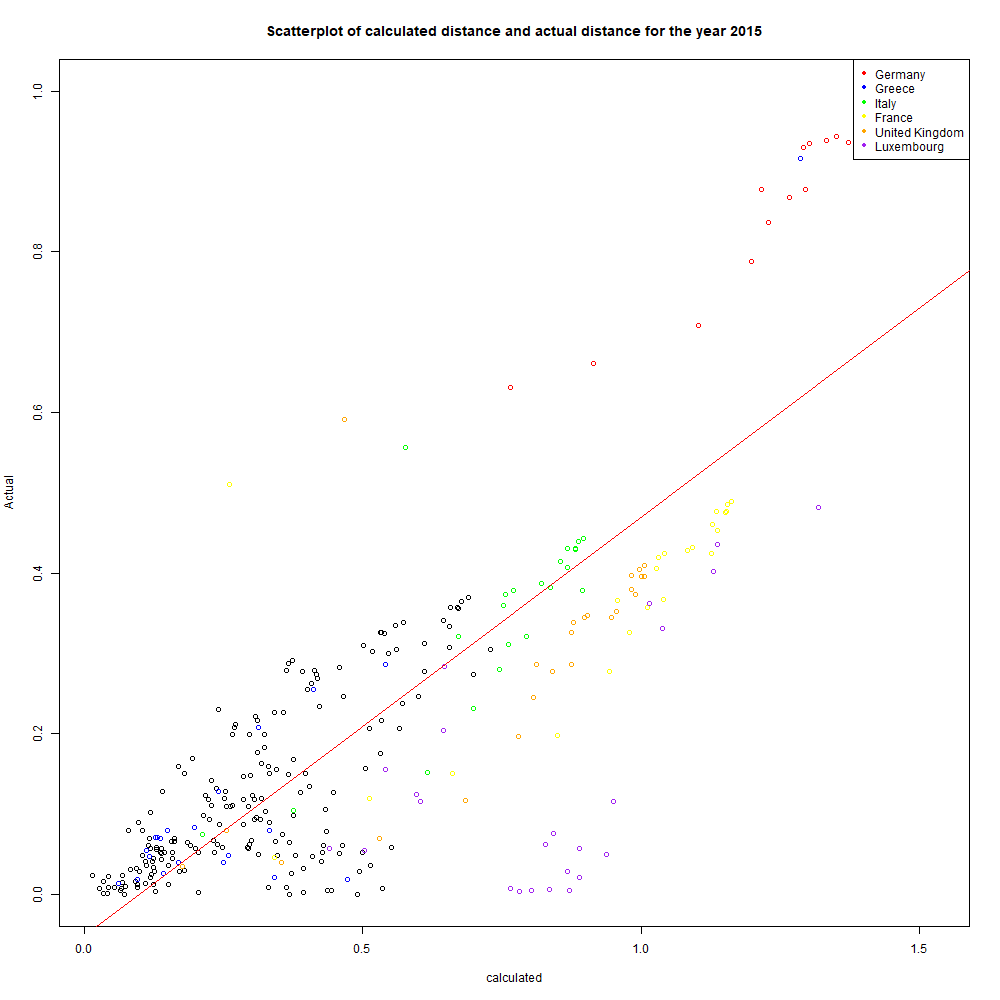
\includegraphics[width = \textwidth]{images/scatterplot_with_regression_line_ 2015 .png}
	Παρατηρήσεις:
	\begin{itemize}
		\item Η πρώτη παρατήρηση είναι πως τα δεδομένα δείχνουν να έχουν μία σχεδόν γραμμική σχέση, με μερικές εξαιρέσεις, όπως το Λουξεμβούργο, τη Γερμανία και τη Γαλλία.
		\item Ακόμα και έτσι, οι χώρες οι οποίες παρεκκλίνουν μοιάζουν σαν να υπακούν μία δική τους γραμμική σχέση με παρόμοια κλίση, αλλά διαφορετική dc συνιστώσα. Το οποίο σημαίνει πως δεν έχουν καταφέρει με τα δεδομένα μας να μαζέψουμε όση πληροφορία χρειάζεται ή πως υπάρχει εγγενώς μία αδικία και η Γερμανία είναι μονίμως ευνοημένη ενώ το Λουξεμβούργο είναι συνεχώς αδικημένο. 
	\end{itemize}
	\subsection{Πείραμα 2}
	Εδώ δοκιμάζουμε για να δούμε αν υπάρχει κάποια σημαντική αλλαγή μέσα στα χρόνια από το 2014 μέχρι το 2019.΄
	\begin{figure}[H]
		\centering
		\begin{subfigure}[b]{0.3\textwidth}
			\centering
			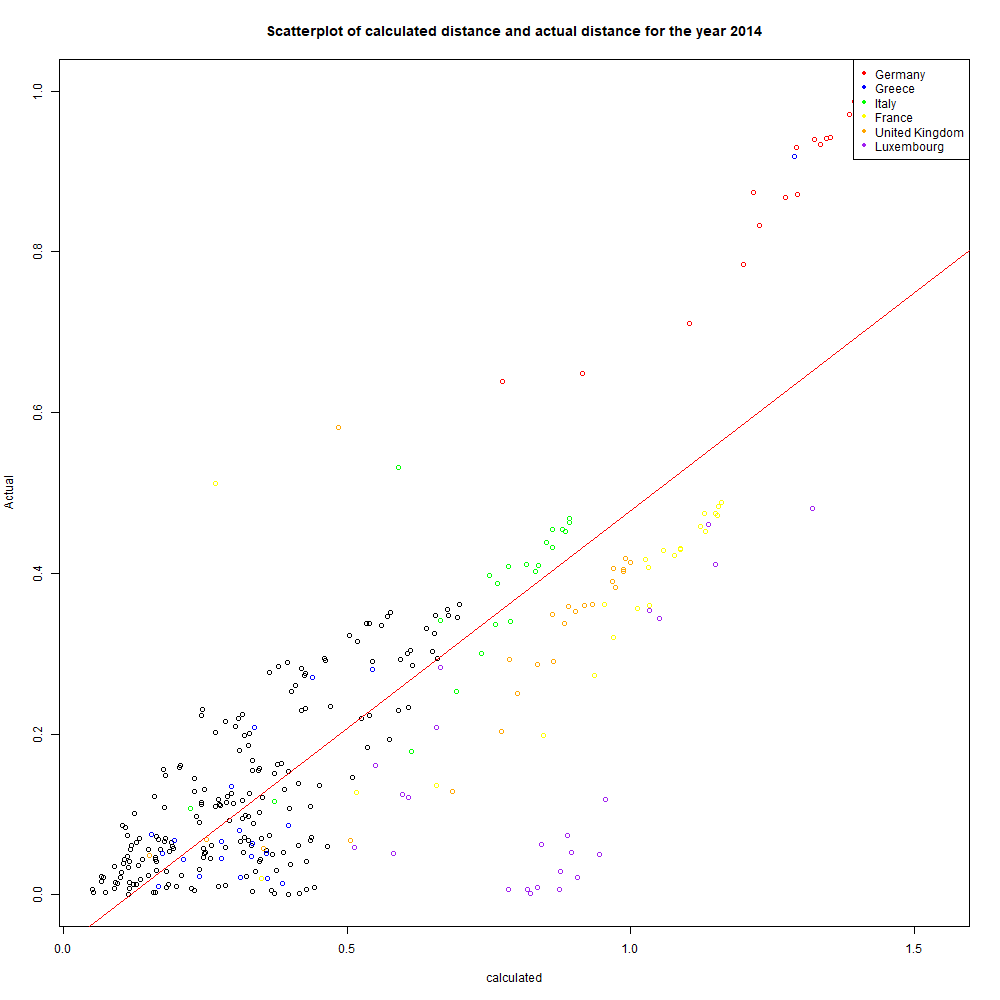
\includegraphics[width=\textwidth]{images/scatterplot_with_regression_line_ 2014 .png}
			\caption{2014}
		\end{subfigure}
		\hfill
		\begin{subfigure}[b]{0.3\textwidth}
			\centering
			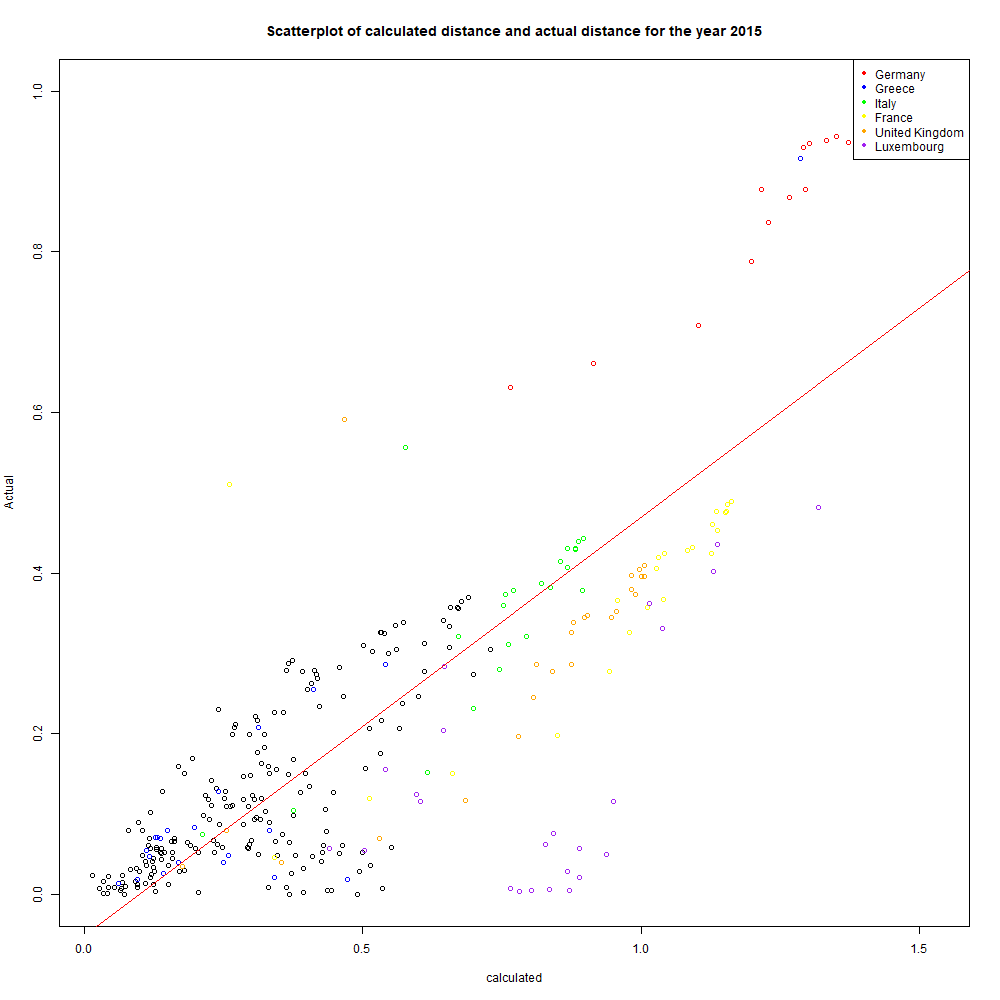
\includegraphics[width=\textwidth]{images/scatterplot_with_regression_line_ 2015 .png}
			\caption{2015}
		\end{subfigure}
		\hfill
		\begin{subfigure}[b]{0.3\textwidth}
			\centering
			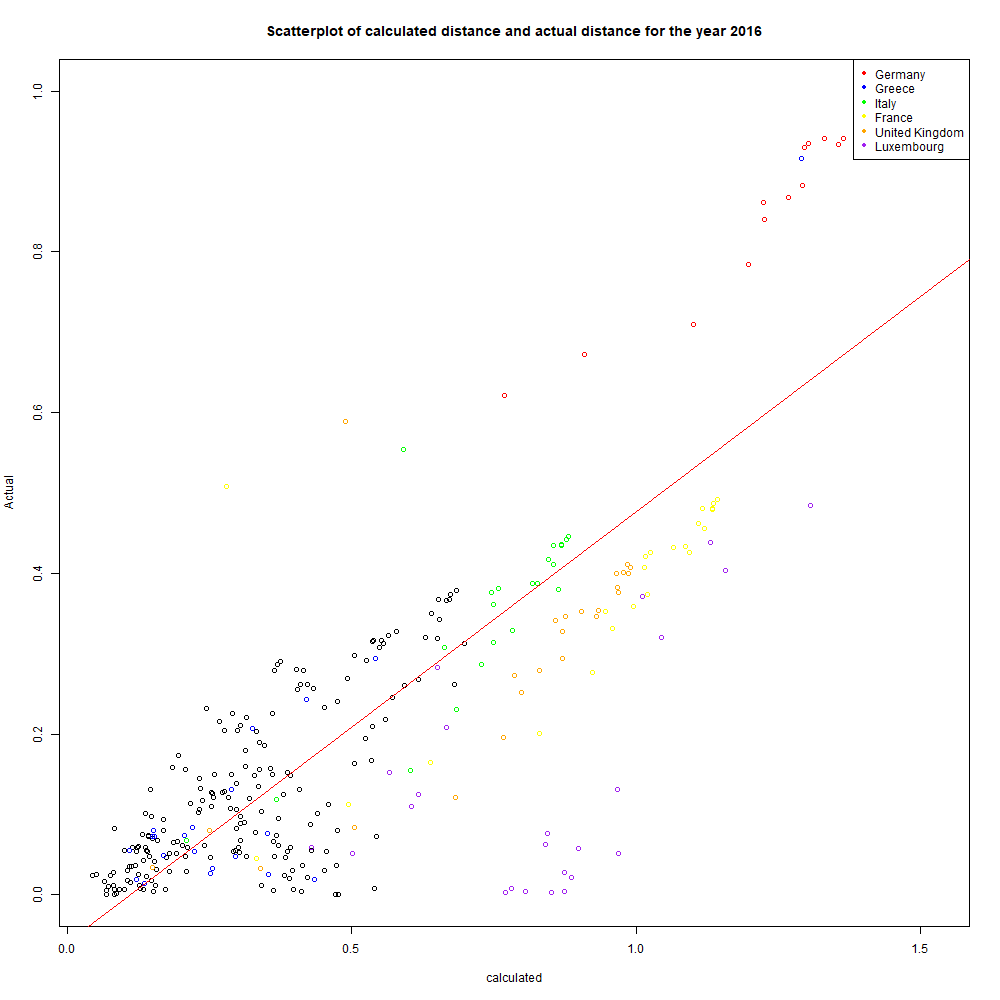
\includegraphics[width=\textwidth]{images/scatterplot_with_regression_line_ 2016 .png}
			\caption{2016}
		\end{subfigure}
		\begin{subfigure}[b]{0.3\textwidth}
			\centering
			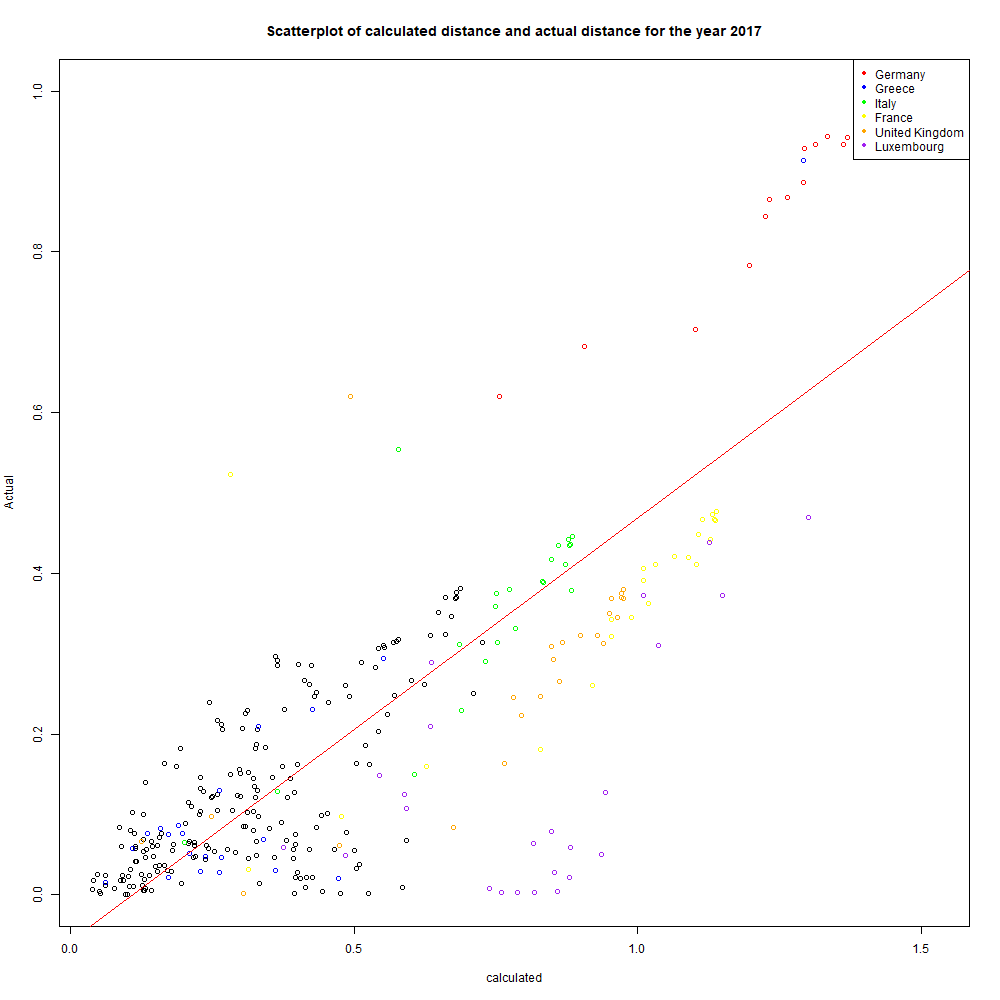
\includegraphics[width=\textwidth]{images/scatterplot_with_regression_line_ 2017 .png}
			\caption{2017}
		\end{subfigure}
		\hfill
		\begin{subfigure}[b]{0.3\textwidth}
			\centering
			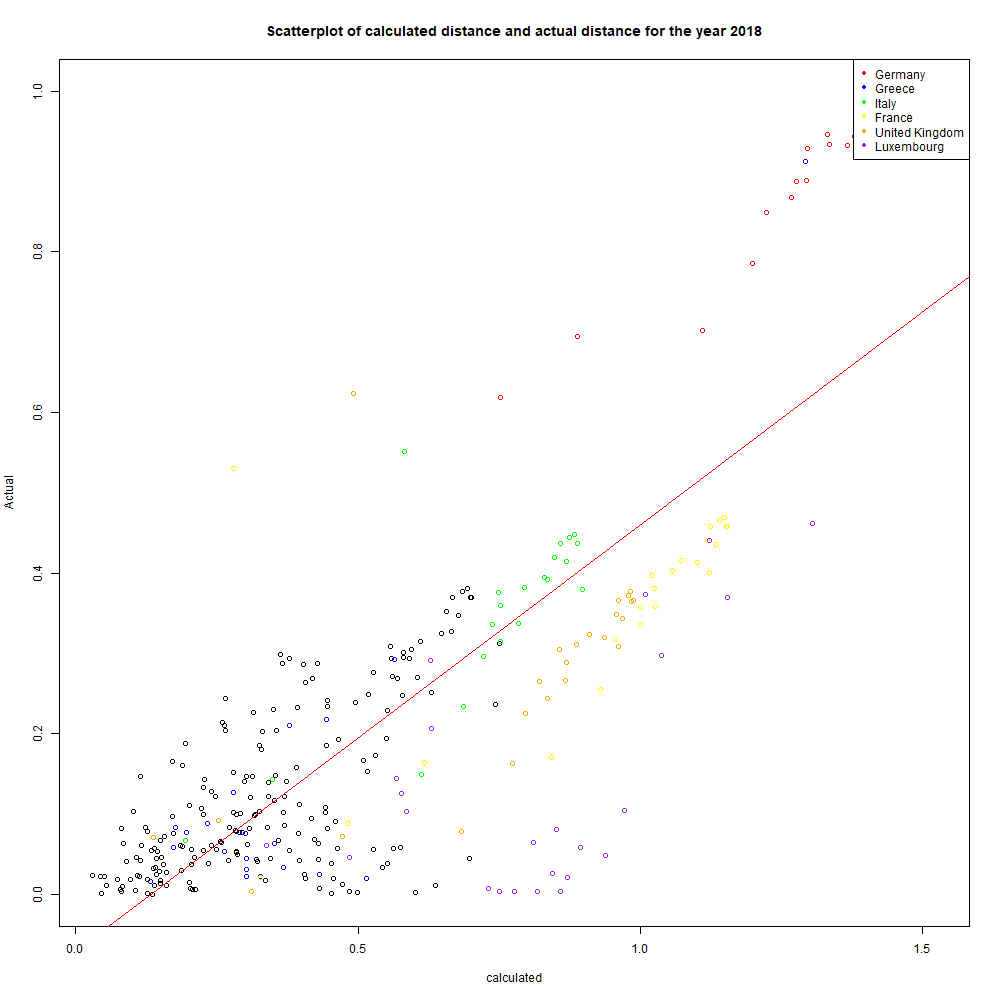
\includegraphics[width=\textwidth]{images/scatterplot_with_regression_line_ 2018 .png}
			\caption{2018}
		\end{subfigure}
		\hfill
		\begin{subfigure}[b]{0.3\textwidth}
			\centering
			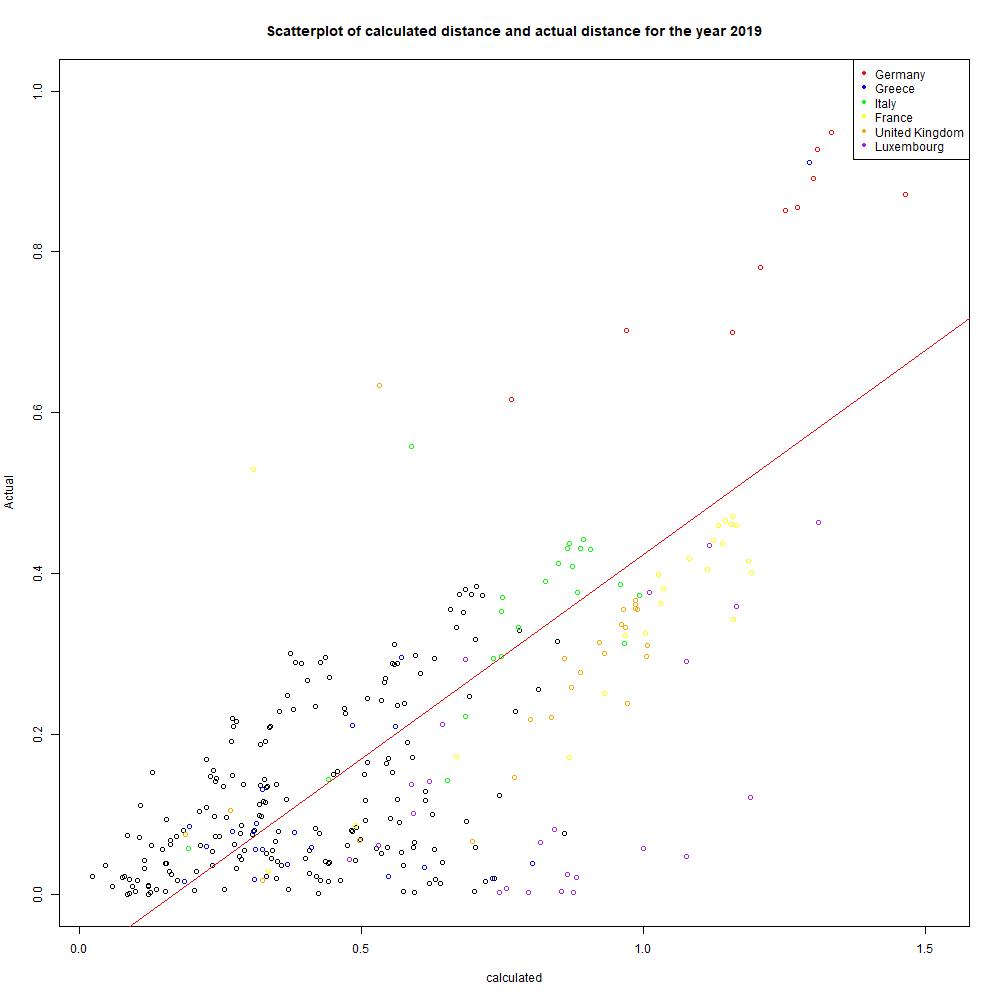
\includegraphics[width=\textwidth]{images/scatterplot_with_regression_line_ 2019 .png}
			\caption{2019}
		\end{subfigure}
		\caption{Συγκριτικό διάγραμμα για το πείραμα 2}
		\label{Συγκριτικό.}
	\end{figure}
	
	\subsection{Πείραμα 3}
	
	Όπως είδαμε ήδη στο πείραμα 1, ή υπάρχει κάποια εγγενής αδικία ή χρειαζόμαστε περισσότερα δεδομένα, τα οποία να κάνουν τις αποστάσεις των χωρών πιο αντιπροσωπευτικές. Για να το πετύχουμε αυτό, συμπεριλάβαμε περισσότερα δεδομένα, τα οποία να μπορούν να δείξουν τη βασική διαφορά μεταξύ του λουξεμβούργου και της Γερμανίας. Τη διαφορά στην κλίμακα της οικονομίας για την οποία μιλάμε. Έτσι βάλαμε 3 μεγέθη τα οποία έχουν να κάνουν και με την ανάπτυξη της οικονομίας αλλά και με τον καταμερισμό της οικονομίας σε διαφορετικούς κλάδους. Φροντίσαμε επίσης, όλα τα νέα στοιχεία να σχετίζονται άμεσα με την παραγωγή διοξειδίου, οπότε για παράδειγμα οι υπηρεσίες της κάθε χώρας αφέθηκαν εκτός. Επίσης, γνωρίζουμε από πριν πως αυτό το μείγμα χαρακτηριστικών δίνει μεγαλύτερη βαρύτητα στο μέγεθος της οικονομίας. Έτσι προκύπτουν τα παρακάτω:
	
	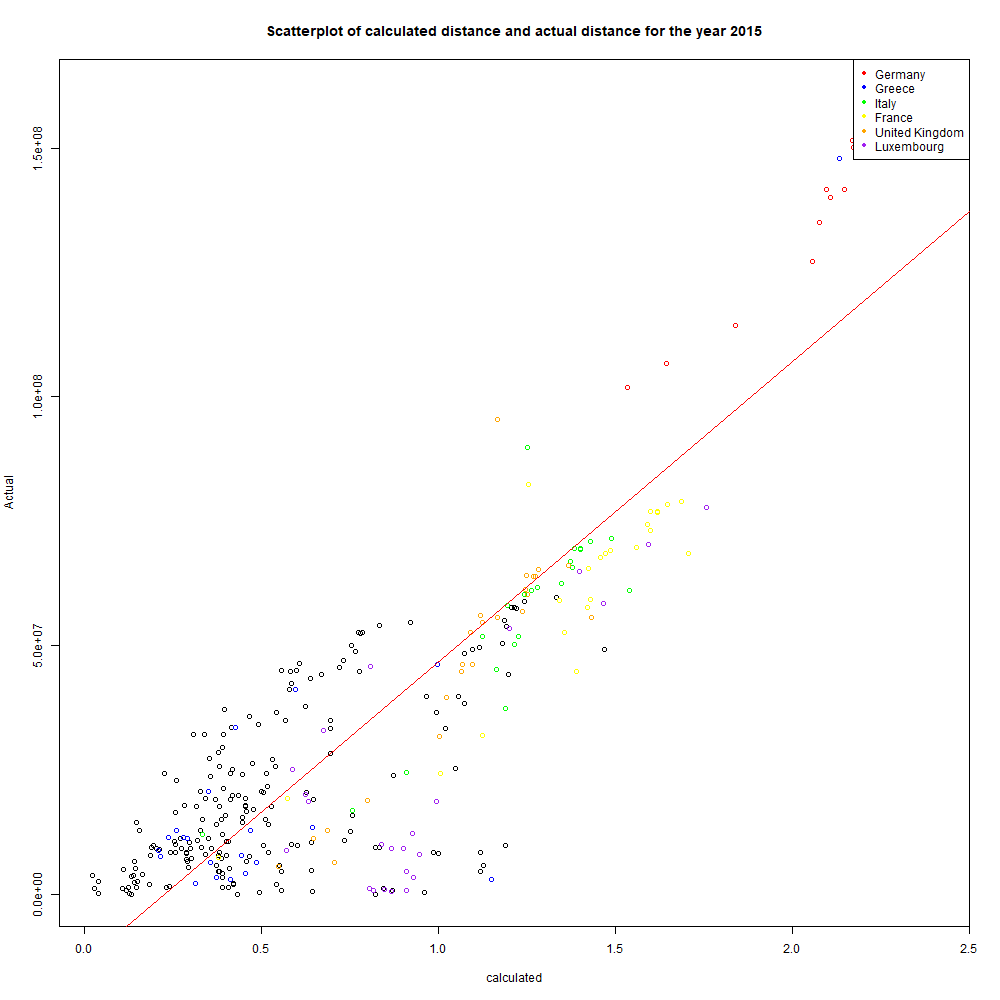
\includegraphics[width = \textwidth]{images/scatterplot_with_regression_line_ 2015 _with_all_data_.png}
	
	Παρατηρήσεις:
	\begin{itemize}
		\item Παρατηρούμε πως όλες οι χώρες έχουν έρθει πιο κοντά στη γραμμή. Όμως αυτό έχει να κάνει περισσότερο με το ότι η Γερμανία βρέθηκε πιο μακριά από τις υπόλοιπες, με αποτέλεσμα να "μειώνεται η ανάλυση" στις μικρότερες χώρες. Συνεπώς, παρόλο που όλα δείχνουν να είναι πιο κοντά στη γραμμή, στην πραγματικότητα απλώς έχουμε "ξεζουμάρει" και το γράφημα είναι παρόμοιο με πριν.
		\item Η προηγούμενη παρατήρηση βέβαια δεν αναιρεί το γεγονός ότι αυτό το μοντέλο όντως καταφέρνει να περιγράψει καλύτερα την Γερμανία. Απλώς χάνει σε όλες τις υπόλοιπες χώρες.
	\end{itemize}
	
	\subsection{Πείραμα 4}
	Βλέποντας την αποτυχία του προηγούμενου μοντέλου, θα προσπαθήσουμε να λογαριθμίσουμε τα πάντα, ώστε να έχουμε περισσότερη ανάλυση στις χαμηλές τιμές και να φέρουμε τη Γερμανία σε πιο χαμηλές τιμές. Έτσι προκύπτει το παρακάτω:
	
	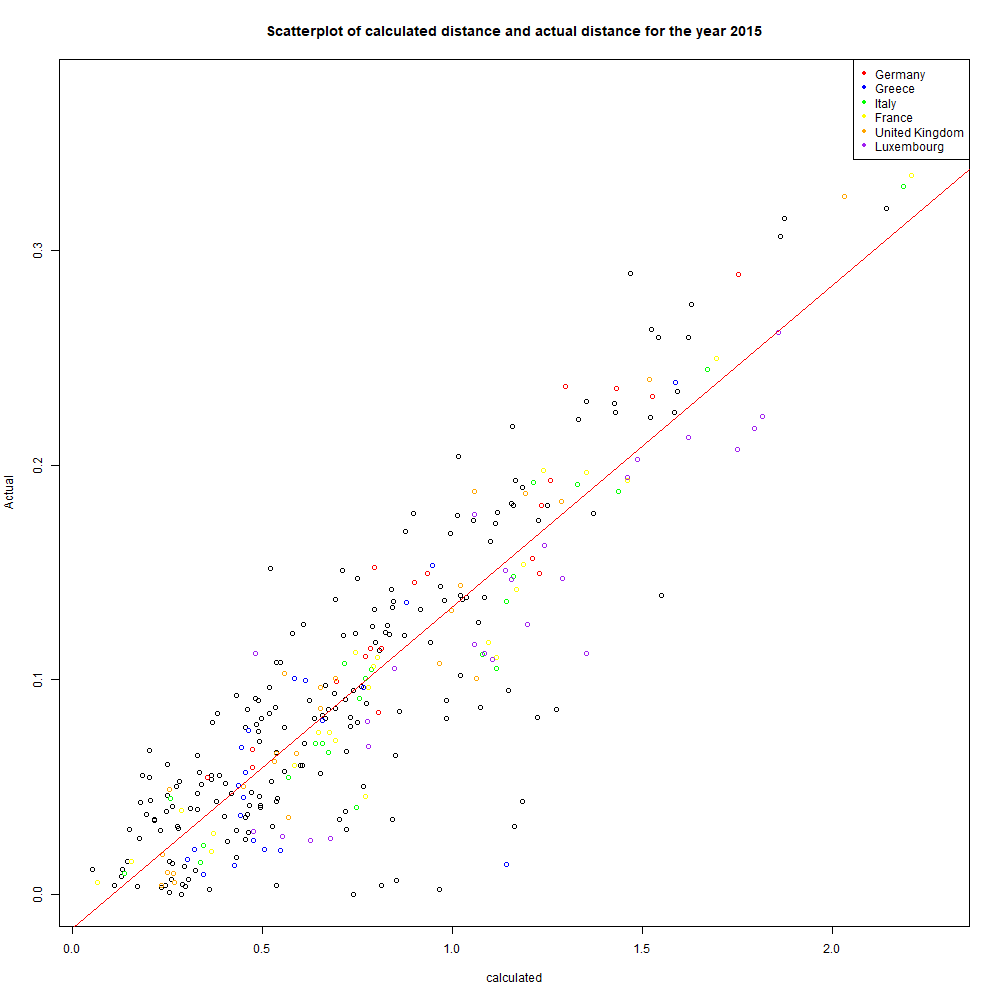
\includegraphics[width = \textwidth]{images/scatterplot_with_regression_line_ 2015 _with_all_data_and_log= TRUE .png}
	Παρατηρήσεις:
	\begin{itemize}
		\item Black Magic.
		\item Πέρα από την πλάκα, είναι σαφές πως εδώ όλα έχουν έρθει αρκετά πιο κοντά όλες οι τιμές. Επομένως, οι ίδιες αποκλίσεις με πριν πλέον σηματοδοτούν ακόμα μεγαλύτερη πραγματική απόσταση.Όμως το αποτέλεσμα δείχνει πως κάποια μορφή τέτοιες "δικαιοσύνης" υπάρχει όντως. 
	\end{itemize}
	
	\section{Προτάσεις}
	
	Αρχικά για να επαναλάβει κάποιος τα πειράματα αυτά θα χρειαστεί την βάση EU ETS και αυτό εδώ το github: https://github.com/kwpap/Diplomatiki\_kwpap\_step\_1
	
	\begin{itemize}
		\item Καλύτερη επιλογή διανυσμάτων.
		\item Βάρη στην κάθε τιμή του κάθε διανύσματος. Εδώ πρέπει βέβαια να δοθεί προσοχή για να αποφύγουμε το overfiting. 
		\item Συζήτηση για μελλοντικά ενδιαφέροντα πράγματα που μπορούν να γίνουν.
		\item Θα ήταν ενδιαφέρον αν σε ένα δεύτερο επίπεδο δε μιλούσαμε πλέον για αποστάσεις, αλλά για απόλυτα νούμερα. Ανεξαρτήτως χώρας και πλέον η αναζήτηση είχε ως σκοπό να βρει τα χαρακτηριστικά εκείνα τα οποία μπορούν να αυξήσουν τις δωρεάν άδειες μίας χώρας.
	\end{itemize}
	\section{Ένθετο}
	Παρακάτω φαίνονται τα χαρακτηριστικά των γραμμικών παλινδρομήσεων:
	\begin{table}[ht]
		\centering
		\begin{tabular}{c|c|c|c|c|c }
			Test & Slope & intercept & Multiple $R^2$ & Adjusted $R^2$ & p-value\\
			\hline
			2014                     & 0.54185&-0.06402     & 0.6968   & 0.6958   &  $<$ 2.2e-16\\
			2015                     &0.52049&  -0.05067    & 0.6823   & 0.6813   &  $<$ 2.2e-16\\
			2016                       &0.53501    & -0.05890   & 0.6916   & 0.6906   &  $<$ 2.2e-16\\
			2017                       &0.52720& -0.05817   & 0.6752   &0.6742    &  $<$ 2.2e-16\\
			2018                       &0.52966& -0.06977   & 0.6625   & 0.6615    &  $<$ 2.2e-16\\
			2019                     &0.50753    & -0.08467     & 0.6008   & 0.5996   &  $<$ 2.2e-16\\
			2015 all data              &60298846&  -13563147      & 0.7886   & 0.788   &   $<$ 2.2e-16\\
			2015 all data + log        &0.149767   &-0.015708       & 0.7977   & 0.7971   &  $<$ 2.2e-16\\
			\hline
			
		\end{tabular}
	\end{table}
	
	\begin{table}[ht]
		\footnotesize
		\centering
		\tabcolsep=0.11cm
		\begin{tabular}{r|rrrrrrrrrr}
			\hline
			& Austria & Belgium & Bulgaria & Croatia & Cyprus & Denmark & Estonia & Finland & France & Germany \\
			\hline
			Austria & 0.00 & 0.18 & 0.49 & 0.64 & 1.12 & 0.26 & 0.83 & 0.17 & 0.69 & 0.77 \\
			Belgium & 0.18 & 0.00 & 0.49 & 0.55 & 1.02 & 0.20 & 0.75 & 0.23 & 0.77 & 0.81 \\
			Bulgaria & 0.49 & 0.49 & 0.00 & 0.40 & 0.79 & 0.54 & 0.49 & 0.47 & 1.09 & 1.21 \\
			Croatia & 0.64 & 0.55 & 0.40 & 0.00 & 0.52 & 0.50 & 0.33 & 0.56 & 1.19 & 1.26 \\
			Cyprus & 1.12 & 1.02 & 0.79 & 0.52 & 0.00 & 0.98 & 0.33 & 1.06 & 1.70 & 1.75 \\
			Denmark & 0.26 & 0.20 & 0.54 & 0.50 & 0.98 & 0.00 & 0.75 & 0.19 & 0.74 & 0.80 \\
			Estonia & 0.83 & 0.75 & 0.49 & 0.33 & 0.33 & 0.75 & 0.00 & 0.80 & 1.46 & 1.53 \\
			Finland & 0.17 & 0.23 & 0.47 & 0.56 & 1.06 & 0.19 & 0.80 & 0.00 & 0.68 & 0.78 \\
			France & 0.69 & 0.77 & 1.09 & 1.19 & 1.70 & 0.74 & 1.46 & 0.68 & 0.00 & 0.29 \\
			Germany & 0.77 & 0.81 & 1.21 & 1.26 & 1.75 & 0.80 & 1.53 & 0.78 & 0.29 & 0.00 \\
			Greece & 0.48 & 0.44 & 0.55 & 0.46 & 0.95 & 0.30 & 0.77 & 0.32 & 0.78 & 0.88 \\
			Hungary & 0.25 & 0.33 & 0.30 & 0.54 & 1.02 & 0.36 & 0.73 & 0.22 & 0.80 & 0.93 \\
			Ireland & 0.72 & 0.85 & 0.85 & 1.18 & 1.55 & 0.97 & 1.22 & 0.84 & 1.12 & 1.23 \\
			Italy & 0.67 & 0.75 & 1.08 & 1.16 & 1.67 & 0.72 & 1.44 & 0.66 & 0.07 & 0.26 \\
			Latvia & 0.79 & 0.71 & 0.49 & 0.18 & 0.37 & 0.66 & 0.23 & 0.71 & 1.35 & 1.43 \\
			Lithuania & 0.61 & 0.52 & 0.41 & 0.05 & 0.54 & 0.46 & 0.34 & 0.54 & 1.17 & 1.23 \\
			Luxembourg & 1.14 & 1.06 & 0.85 & 0.78 & 0.55 & 1.11 & 0.48 & 1.15 & 1.81 & 1.86 \\
			Malta & 1.52 & 1.47 & 1.16 & 1.16 & 0.86 & 1.52 & 0.84 & 1.54 & 2.21 & 2.27 \\
			Netherlands & 0.38 & 0.43 & 0.77 & 0.83 & 1.33 & 0.38 & 1.10 & 0.33 & 0.37 & 0.47 \\
			Poland & 0.40 & 0.46 & 0.76 & 0.84 & 1.35 & 0.43 & 1.11 & 0.36 & 0.37 & 0.47 \\
			Portugal & 0.21 & 0.25 & 0.32 & 0.47 & 0.97 & 0.26 & 0.69 & 0.15 & 0.79 & 0.90 \\
			Romania & 0.30 & 0.43 & 0.49 & 0.73 & 1.23 & 0.46 & 0.94 & 0.29 & 0.65 & 0.81 \\
			Slovenia & 0.61 & 0.52 & 0.37 & 0.21 & 0.52 & 0.52 & 0.24 & 0.58 & 1.24 & 1.30 \\
			Spain & 0.65 & 0.72 & 1.02 & 1.08 & 1.59 & 0.66 & 1.37 & 0.60 & 0.15 & 0.36 \\
			Sweden & 0.13 & 0.26 & 0.56 & 0.69 & 1.18 & 0.28 & 0.92 & 0.14 & 0.58 & 0.69 \\
			United Kingdom & 0.53 & 0.57 & 0.97 & 1.02 & 1.52 & 0.56 & 1.29 & 0.54 & 0.27 & 0.25 \\
			\hline
		\end{tabular}
		\caption{Distance between countries in 2015, part 1}
		\label{tab:distance_2015}
	\end{table}
	
	\begin{table}[ht]
		\footnotesize
		\centering
		\tabcolsep=0.11cm
		\begin{tabular}{r|rrrrrrrrrr}
			\hline
			& Greece & Hungary & Ireland & Italy & Latvia & Lithuania & Luxembourg & Malta & Netherlands & Poland \\
			\hline
			Austria & 0.48 & 0.25 & 0.72 & 0.67 & 0.79 & 0.61 & 1.14 & 1.52 & 0.38 & 0.40 \\
			Belgium & 0.44 & 0.33 & 0.85 & 0.75 & 0.71 & 0.52 & 1.06 & 1.47 & 0.43 & 0.46 \\
			Bulgaria & 0.55 & 0.30 & 0.85 & 1.08 & 0.49 & 0.41 & 0.85 & 1.16 & 0.77 & 0.76 \\
			Croatia & 0.46 & 0.54 & 1.18 & 1.16 & 0.18 & 0.05 & 0.78 & 1.16 & 0.83 & 0.84 \\
			Cyprus & 0.95 & 1.02 & 1.55 & 1.67 & 0.37 & 0.54 & 0.55 & 0.86 & 1.33 & 1.35 \\
			Denmark & 0.30 & 0.36 & 0.97 & 0.72 & 0.66 & 0.46 & 1.11 & 1.52 & 0.38 & 0.43 \\
			Estonia & 0.77 & 0.73 & 1.22 & 1.44 & 0.23 & 0.34 & 0.48 & 0.84 & 1.10 & 1.11 \\
			Finland & 0.32 & 0.22 & 0.84 & 0.66 & 0.71 & 0.54 & 1.15 & 1.54 & 0.33 & 0.36 \\
			France & 0.78 & 0.80 & 1.12 & 0.07 & 1.35 & 1.17 & 1.81 & 2.21 & 0.37 & 0.37 \\
			Germany & 0.88 & 0.93 & 1.23 & 0.26 & 1.43 & 1.23 & 1.86 & 2.27 & 0.47 & 0.47 \\
			Greece & 0.00 & 0.43 & 1.14 & 0.75 & 0.61 & 0.45 & 1.20 & 1.59 & 0.45 & 0.46 \\
			Hungary & 0.43 & 0.00 & 0.74 & 0.79 & 0.67 & 0.53 & 1.08 & 1.43 & 0.50 & 0.49 \\
			Ireland & 1.14 & 0.74 & 0.00 & 1.12 & 1.27 & 1.16 & 1.35 & 1.58 & 0.98 & 0.98 \\
			Italy & 0.75 & 0.79 & 1.12 & 0.00 & 1.33 & 1.14 & 1.79 & 2.19 & 0.34 & 0.34 \\
			Latvia & 0.61 & 0.67 & 1.27 & 1.33 & 0.00 & 0.20 & 0.68 & 1.04 & 1.00 & 1.01 \\
			Lithuania & 0.45 & 0.53 & 1.16 & 1.14 & 0.20 & 0.00 & 0.78 & 1.17 & 0.81 & 0.82 \\
			Luxembourg & 1.20 & 1.08 & 1.35 & 1.79 & 0.68 & 0.78 & 0.00 & 0.48 & 1.46 & 1.49 \\
			Malta & 1.59 & 1.43 & 1.58 & 2.19 & 1.04 & 1.17 & 0.48 & 0.00 & 1.86 & 1.87 \\
			Netherlands & 0.45 & 0.50 & 0.98 & 0.34 & 1.00 & 0.81 & 1.46 & 1.86 & 0.00 & 0.13 \\
			Poland & 0.46 & 0.49 & 0.98 & 0.34 & 1.01 & 0.82 & 1.49 & 1.87 & 0.13 & 0.00 \\
			Portugal & 0.34 & 0.11 & 0.81 & 0.77 & 0.62 & 0.46 & 1.06 & 1.43 & 0.46 & 0.46 \\
			Romania & 0.51 & 0.21 & 0.70 & 0.64 & 0.87 & 0.72 & 1.29 & 1.62 & 0.42 & 0.39 \\
			Slovenia & 0.58 & 0.53 & 1.07 & 1.21 & 0.25 & 0.18 & 0.63 & 1.03 & 0.88 & 0.90 \\
			Spain & 0.66 & 0.74 & 1.15 & 0.14 & 1.25 & 1.07 & 1.75 & 2.14 & 0.30 & 0.29 \\
			Sweden & 0.44 & 0.27 & 0.77 & 0.57 & 0.84 & 0.67 & 1.24 & 1.63 & 0.28 & 0.31 \\
			United Kingdom & 0.65 & 0.69 & 1.06 & 0.23 & 1.19 & 1.00 & 1.62 & 2.03 & 0.24 & 0.25 \\
			\hline
		\end{tabular}
		\caption{Distance between countries in 2015, part 2}
		\label{tab:distance_2015}
	\end{table}
	
	\begin{table}[ht]
		\footnotesize
		\centering
		
		\begin{tabular}{r|rrrrrr}
			\hline
			& Portugal & Romania & Slovenia & Spain & Sweden & United Kingdom \\
			\hline
			Austria & 0.21 & 0.30 & 0.61 & 0.65 & 0.13 & 0.53 \\
			Belgium & 0.25 & 0.43 & 0.52 & 0.72 & 0.26 & 0.57 \\
			Bulgaria & 0.32 & 0.49 & 0.37 & 1.02 & 0.56 & 0.97 \\
			Croatia & 0.47 & 0.73 & 0.21 & 1.08 & 0.69 & 1.02 \\
			Cyprus & 0.97 & 1.23 & 0.52 & 1.59 & 1.18 & 1.52 \\
			Denmark & 0.26 & 0.46 & 0.52 & 0.66 & 0.28 & 0.56 \\
			Estonia & 0.69 & 0.94 & 0.24 & 1.37 & 0.92 & 1.29 \\
			Finland & 0.15 & 0.29 & 0.58 & 0.60 & 0.14 & 0.54 \\
			France & 0.79 & 0.65 & 1.24 & 0.15 & 0.58 & 0.27 \\
			Germany & 0.90 & 0.81 & 1.30 & 0.36 & 0.69 & 0.25 \\
			Greece & 0.34 & 0.51 & 0.58 & 0.66 & 0.44 & 0.65 \\
			Hungary & 0.11 & 0.21 & 0.53 & 0.74 & 0.27 & 0.69 \\
			Ireland & 0.81 & 0.70 & 1.07 & 1.15 & 0.77 & 1.06 \\
			Italy & 0.77 & 0.64 & 1.21 & 0.14 & 0.57 & 0.23 \\
			Latvia & 0.62 & 0.87 & 0.25 & 1.25 & 0.84 & 1.19 \\
			Lithuania & 0.46 & 0.72 & 0.18 & 1.07 & 0.67 & 1.00 \\
			Luxembourg & 1.06 & 1.29 & 0.63 & 1.75 & 1.24 & 1.62 \\
			Malta & 1.43 & 1.62 & 1.03 & 2.14 & 1.63 & 2.03 \\
			Netherlands & 0.46 & 0.42 & 0.88 & 0.30 & 0.28 & 0.24 \\
			Poland & 0.46 & 0.39 & 0.90 & 0.29 & 0.31 & 0.25 \\
			Portugal & 0.00 & 0.28 & 0.48 & 0.72 & 0.25 & 0.65 \\
			Romania & 0.28 & 0.00 & 0.74 & 0.60 & 0.25 & 0.59 \\
			Slovenia & 0.48 & 0.74 & 0.00 & 1.15 & 0.69 & 1.06 \\
			Spain & 0.72 & 0.60 & 1.15 & 0.00 & 0.54 & 0.27 \\
			Sweden & 0.25 & 0.25 & 0.69 & 0.54 & 0.00 & 0.45 \\
			United Kingdom & 0.65 & 0.59 & 1.06 & 0.27 & 0.45 & 0.00 \\
			\hline
		\end{tabular}
		\caption{Distance between countries in 2015, part 3}
		\label{tab:distance_2015}
	\end{table}
	
	Στα γραφήματα \ref{fig:three graphs} φαίνονται κάποιες από τις διαφορές των χωρών σε μία κλίμακα στην οποία το μπλε είνα η μικρότερη απόσταση και το κόκκινο είναι η μεγαλύτερη απόσταση. 
	\begin{figure}[H]
		\centering
		\begin{subfigure}[b]{0.3\textwidth}
			\centering
			\includegraphics[width=\textwidth]{images/heatmap_actual_distances.png}
			\caption{Με βάση τα free.}
			\label{fig:y equals x}
		\end{subfigure}
		\hfill
		\begin{subfigure}[b]{0.3\textwidth}
			\centering
			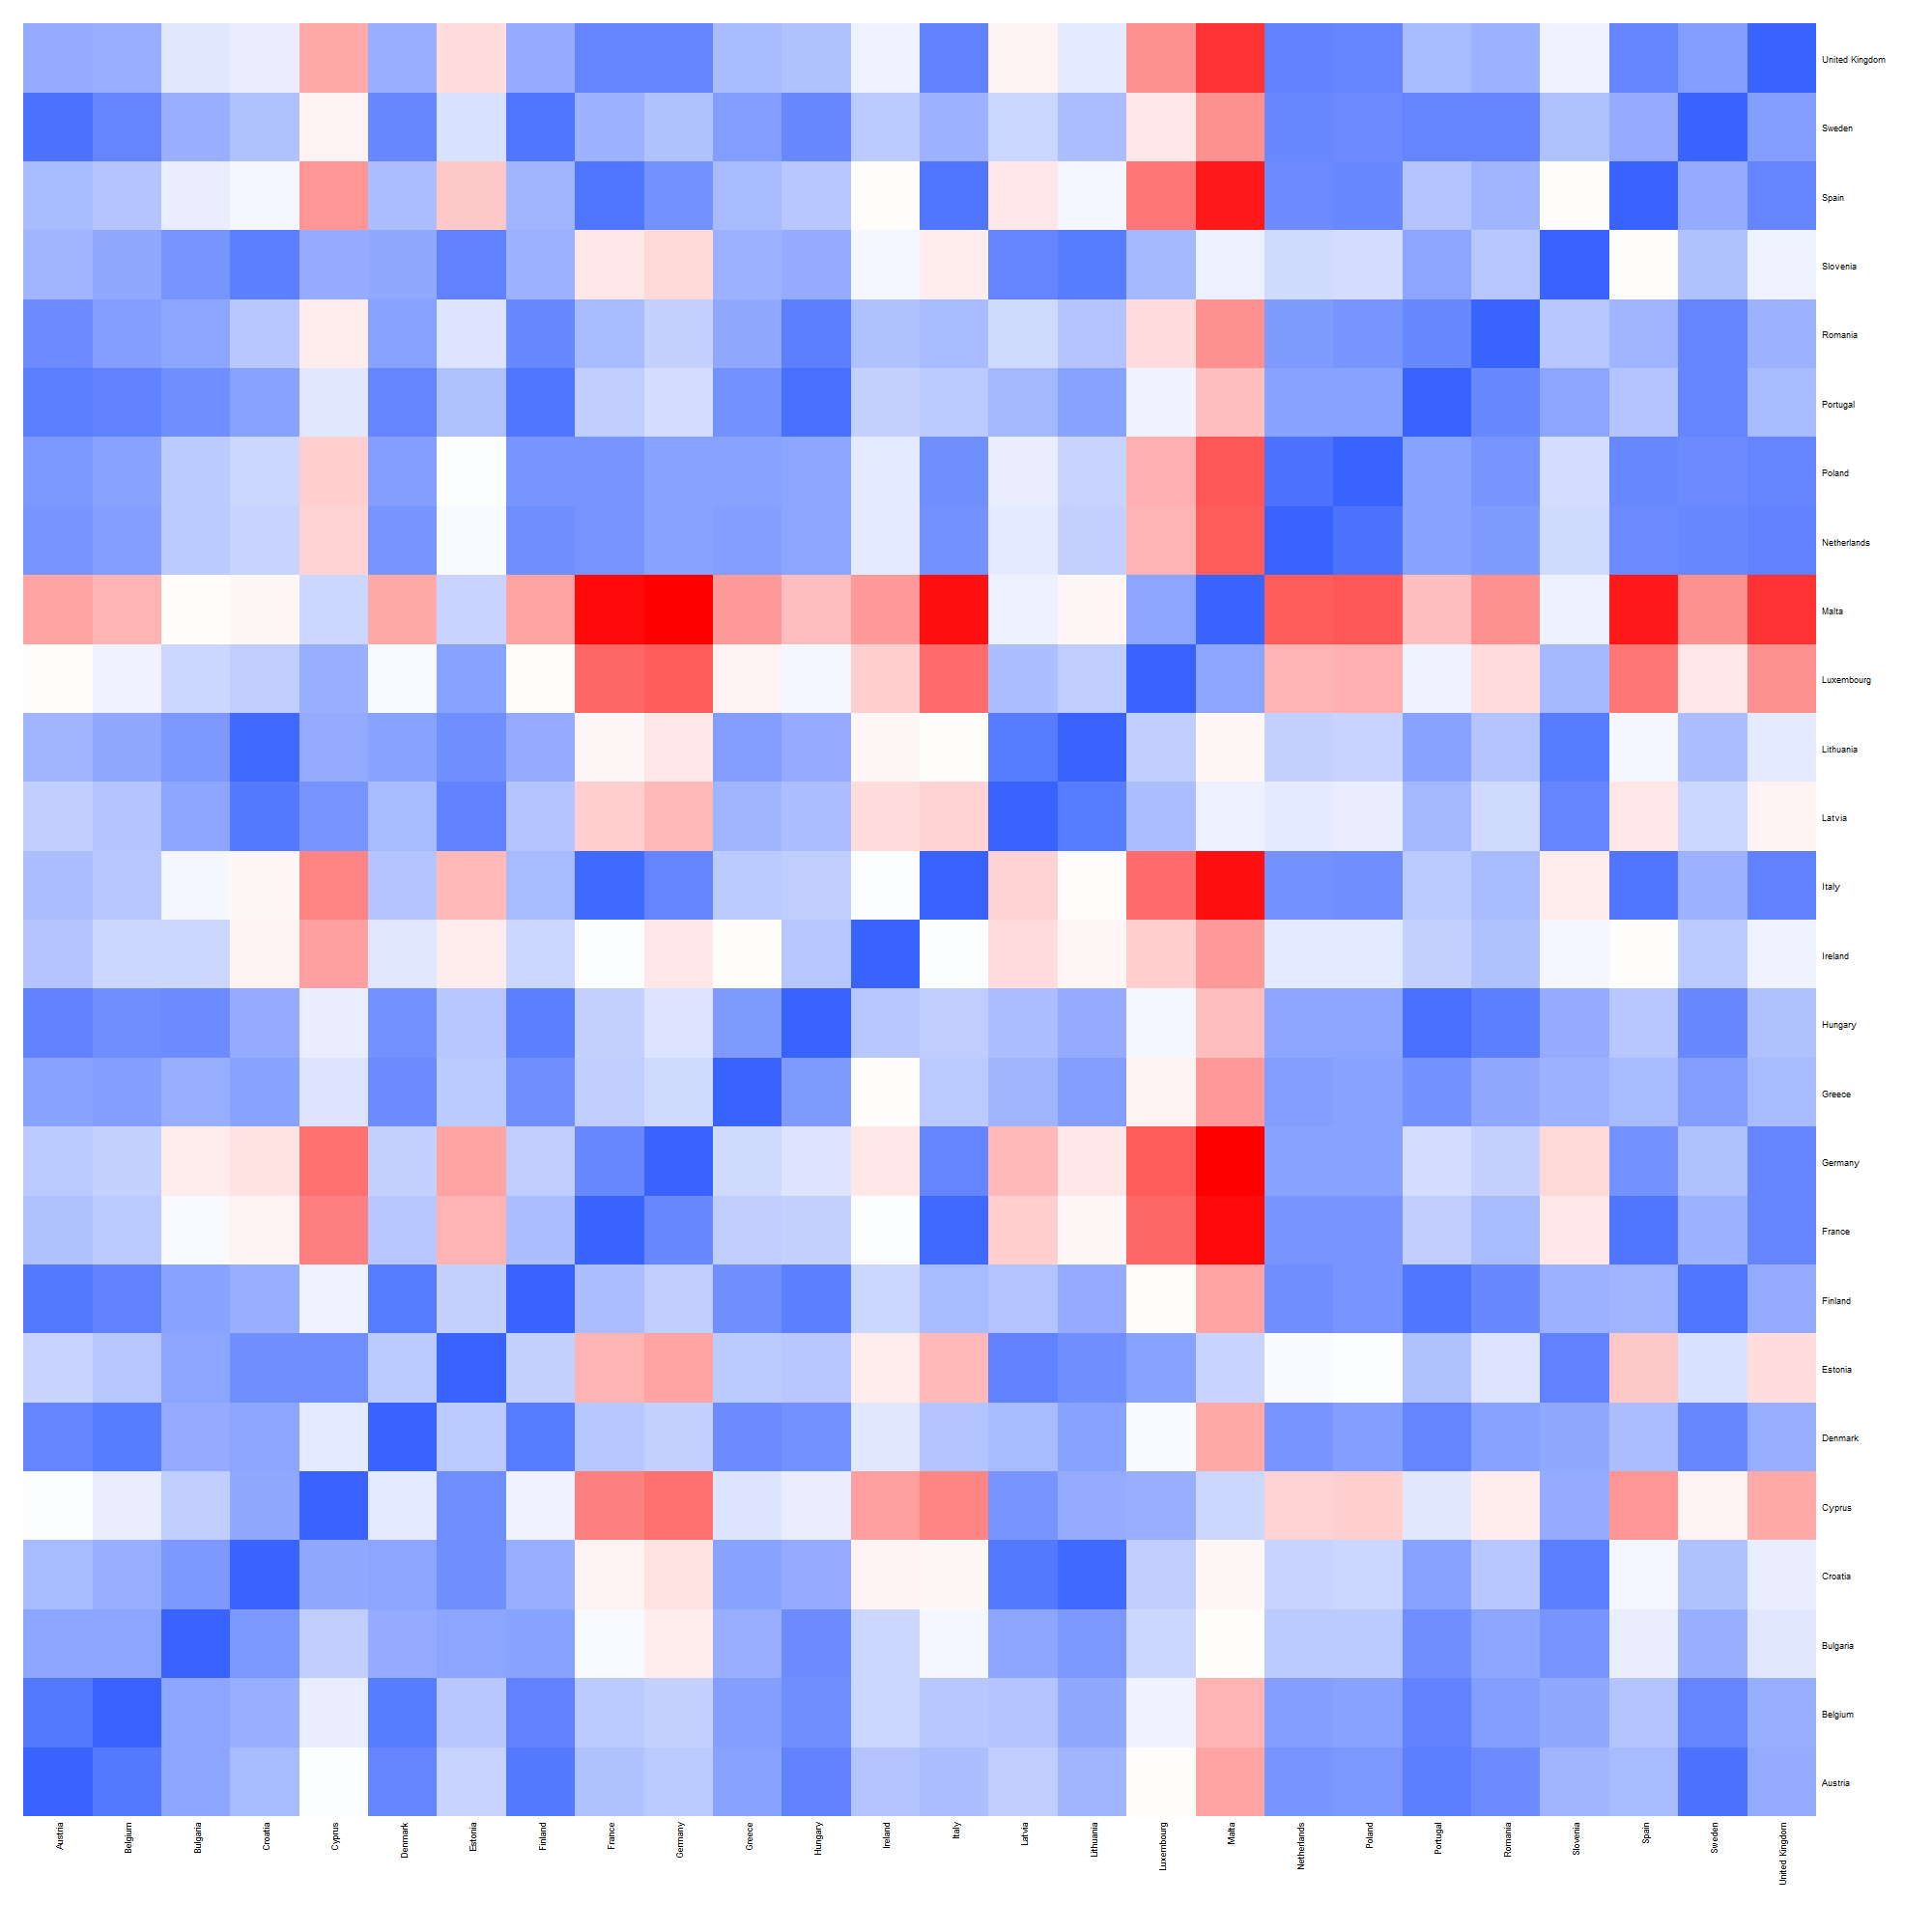
\includegraphics[width=\textwidth]{images/heatmap_distances_of_2015with_full_data_and_log=TRUE.png}
			\caption{Με βάση το διάνυσμα χώρα$_2$ και λογαριθμημένα δεδομένα.}
			\label{fig:three sin x}
		\end{subfigure}
		\hfill
		\begin{subfigure}[b]{0.3\textwidth}
			\centering
			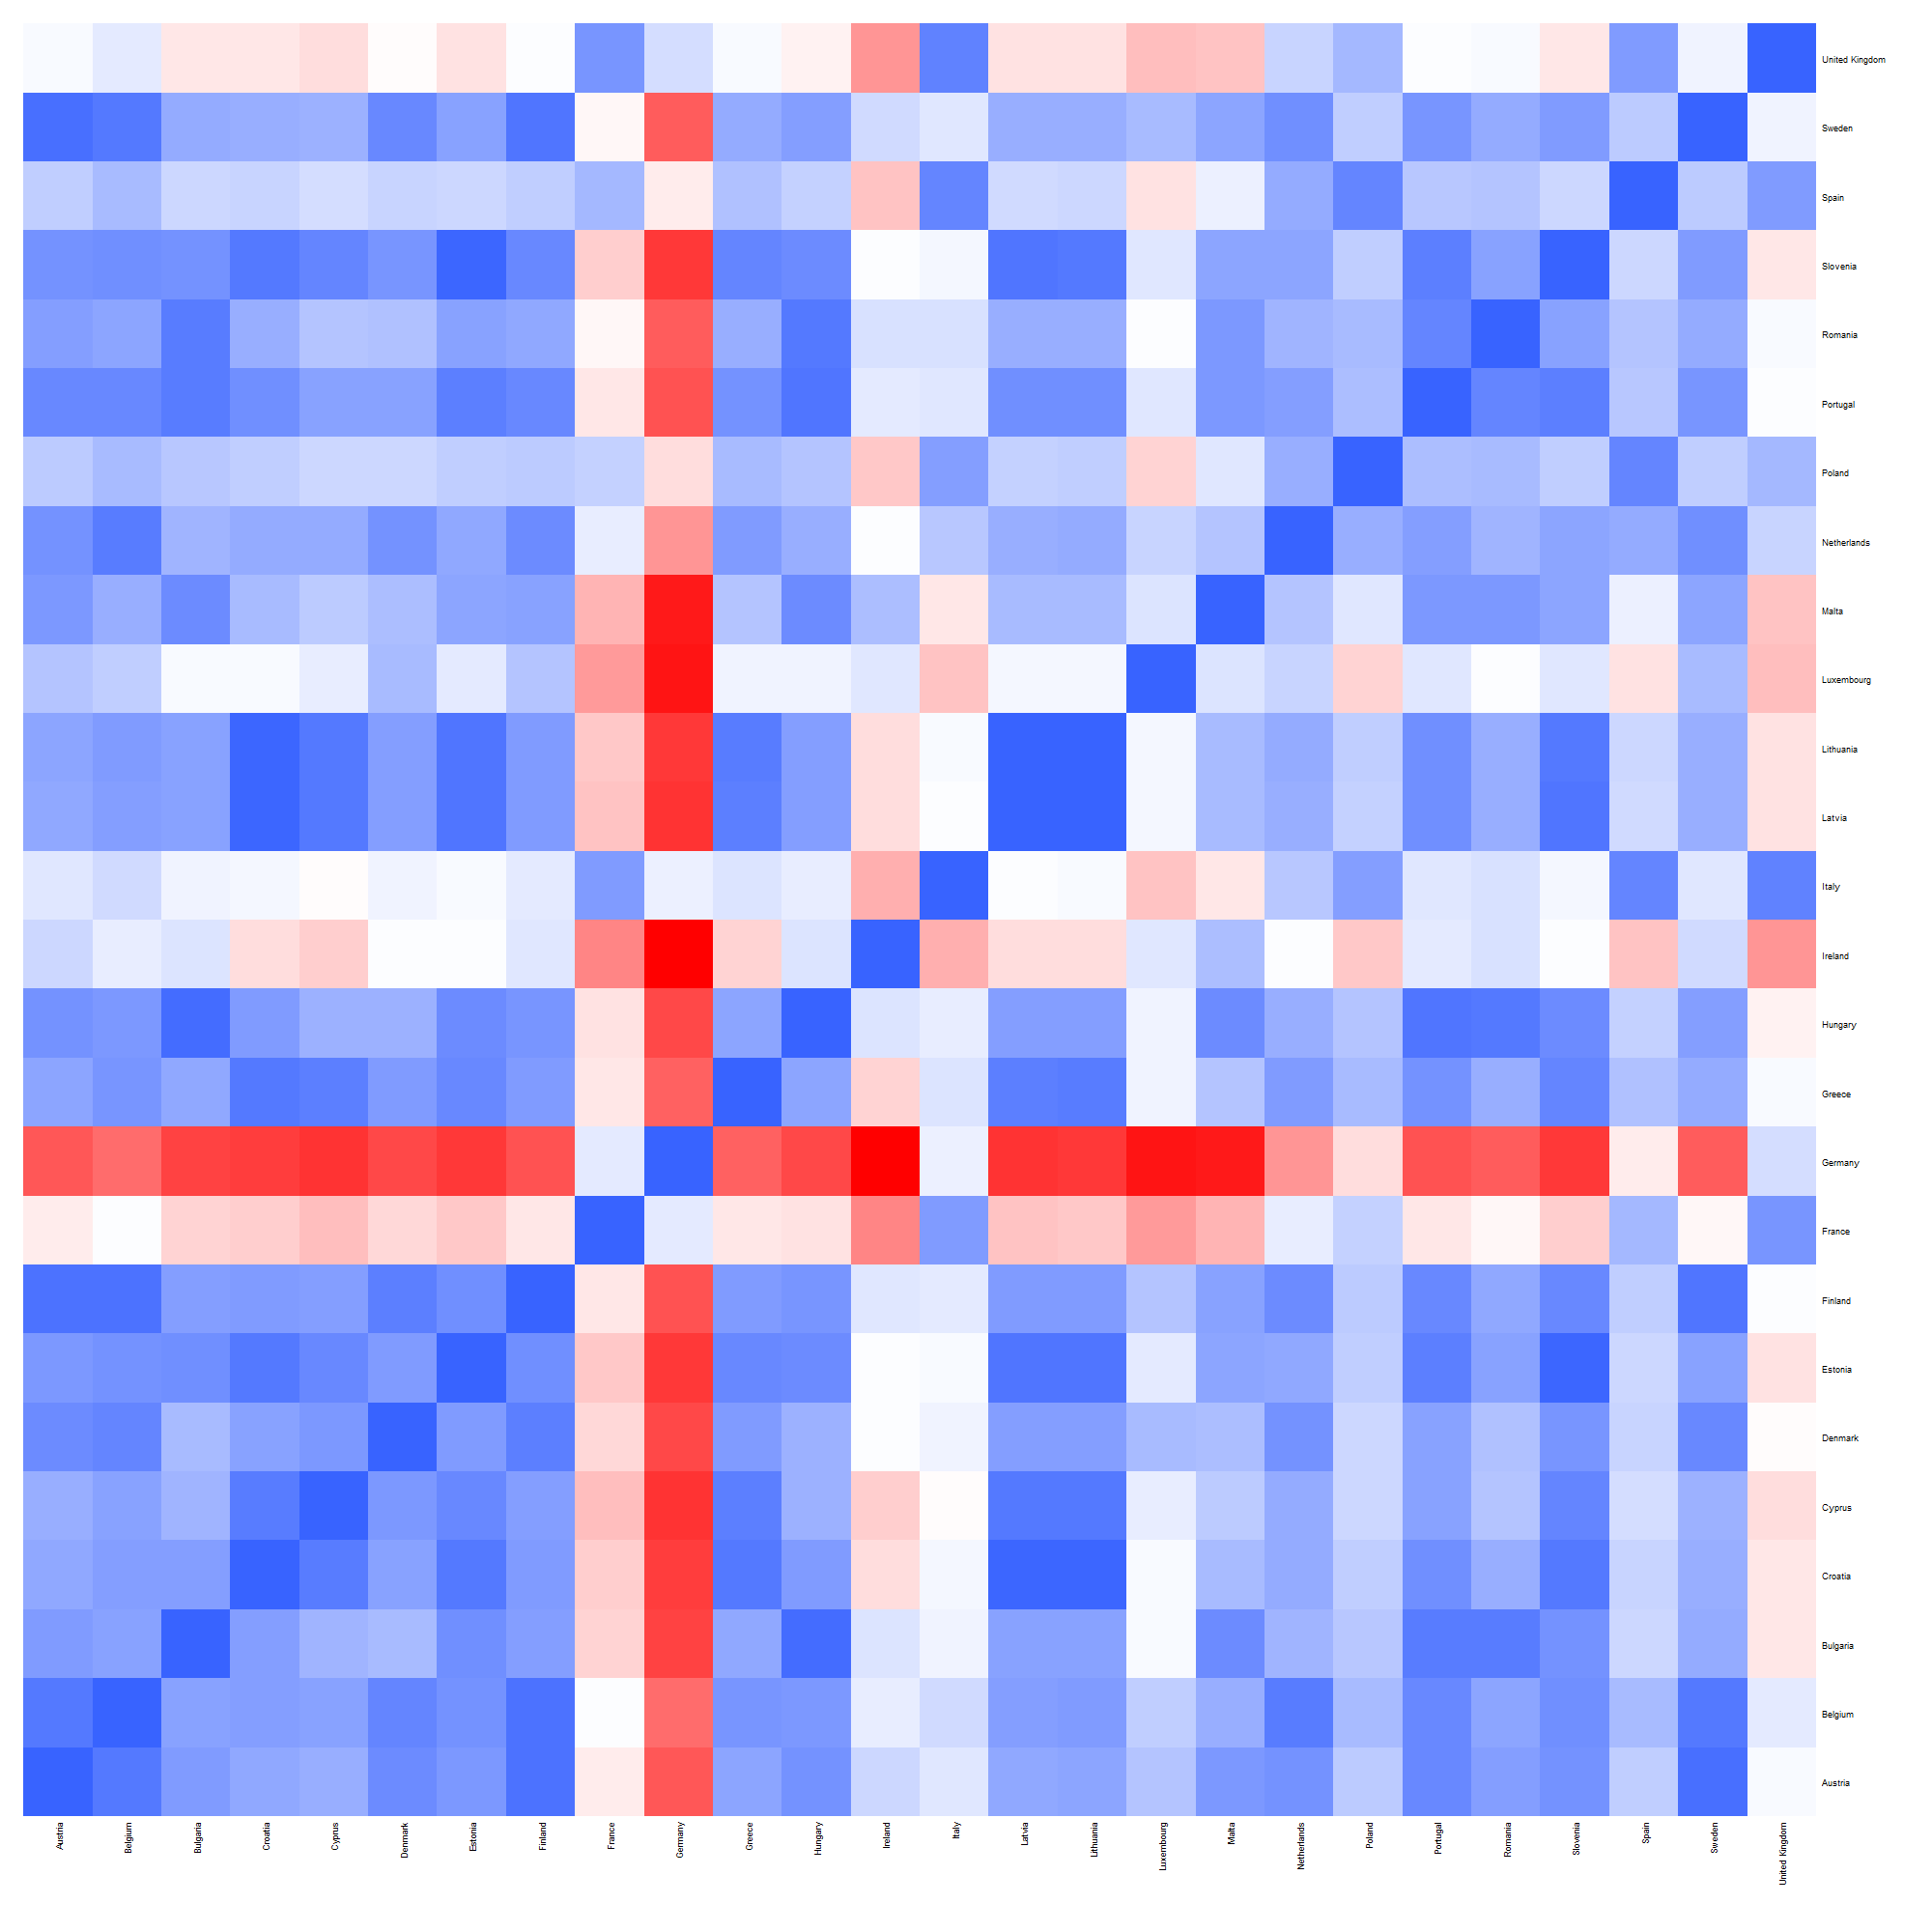
\includegraphics[width=\textwidth]{images/heatmap_distances_of_2015.png}
			\caption{Με βάση το διάνυσμα χώρα$_1$.}
			\label{fig:five over x}
		\end{subfigure}
		\caption{Αποστάσεις χωρών σε heatmap}
		\label{fig:three graphs}
	\end{figure}
	\section{Επανεκίνηση μετά τα Χριστούγεννα}
	Έγινε μία καλύτερη επιλογή των πηγών για τα δεδομένα, το οποίο οδήγησε, χωρίς να μπορώ να το εξηγήσω σε κάτι πολύ περίεργες συμπεριφορές.
	Τα καινούρια δεδομένα ήταν τα:
	\begin{enumerate}
		\item population ίδιο
		\item GDP per capita ίδιο
		\item Total energy supply ίδιο
		\item inflation ίδιο
		\item verified emissions ίδιο
		\item manufacturing σε δiσεκατομύρια δολλάρια, άλλαξε και πλέον δεν έχουμε δεδομένα μόνο για 2010 και 2020, αλλά έχουμε ξεχωριστά για κάθε χρονιά
		\item industry σε δiεκατομύρια δολλάρια, ομοίως
		\item Agricalture σε δiσεκατομύρια δολλάρια, ομοίως
	\end{enumerate}
	Ένα πιθανό πρόβλημα το οποίο ίσως προκύπτει είναι το ότι $(6+7+8) \approx 1*2$. Όμως ρεαλιστικά: $1*2 - (6+7+8) \approx $services. Οπότε ελπίζω πως αυτό δεν είναι σοβαρό πρόβλημα. 
	
	Το δεύτερο που παρατηρώ είναι πως για κάποιο λόγο μετά τις βελτιώσεις στον κώδικα, πλέον αν βάλω τα δεδομένα απλώς να λογαριθμιστούν, τα αποτελέσματα είναι λογικά. Αν βάλω τα αποτελέσματα να κανονικοποιηθούν, πάλι είναι λογικά, αλλά προσεγγίζουν λιγότερο την ευθεία γραμμή. Αν όμως τα βάλω και τα δύο, τότε τα δεδομένα δείχνουν να μην έχουν κάποια γραμμική συσχέτιση, το οποίο δεν το καταλαβαίνω. 
	
	Επίσης, λόγω έλειψης δεδομένων για την παραγωγή της Βουλγαρίας, τα δεδομένα υπολογίστηκαν ως GDP - Agriculture - services - industry.
	
	\section{Δοκιμές για διαφορετικά βάρη στις παραμέτρους}
	Ξέρω πως δεν είπαμε να κάνω αυτό, αλλά όταν ξεκίνησα να το κάνω, δεν μπορούσα να σταματήσω τις δοκιμές. Αρχικά. Όλα όσα θα παρουσιαστούν παρακάτω είναι έχοντας ενεργοποιημένη μόνο την κανονικοποίηση και όχι την λογαρίθμηση, γιατί για αυτήν είχα απορία. 
	
	Για να κρίνω το πόσο σωστά είναι τα βάρη, διάλεξα να προσπαθώ να μεγιστοποιήσω το r squared της παλινδρόμησης. Εγιναν λοιπόν οι παρακάτω δοκιμές:
	\begin{table}[H]
		\begin{tabular}{|llllllll|l|}
			\hline
			Population & \begin{tabular}[c]{@{}l@{}}GDP\\ pe\\ rCapita\end{tabular} & Inflation & \begin{tabular}[c]{@{}l@{}}Agriculture\\  GDP\end{tabular} & \begin{tabular}[c]{@{}l@{}}Industry\\  GDP\end{tabular} & \begin{tabular}[c]{@{}l@{}}Manufacturing\\  GDP\end{tabular} & \begin{tabular}[c]{@{}l@{}}Total\\  Energy\\  Supply\end{tabular} & \begin{tabular}[c]{@{}l@{}}Verified\\  emissions\end{tabular} & r\textasciicircum{}2 \\ \hline
			1          & 1                                                          & 1         & 1                                                          & 1                                                       & 1                                                            & 1                                                                 & 1                                                             & 0.76                 \\
			4          & 0                                                          & 0         & 0                                                          & 10                                                      & 0                                                            & 3                                                                 & 10                                                            & 0.93                 \\
			0          & 0                                                          & 0         & 0                                                          & 6.8                                                     & 0                                                            & 3.2                                                               & 10                                                            & 0.9496               \\
			100        & 0                                                          & 0         & 50                                                         & 626                                                     & 0                                                            & 400                                                               & 1000                                                          & 0.9483               \\
			0          & 0                                                          & 0         & 60                                                         & 570                                                     & 0                                                            & 360                                                               & 981                                                           & 0.953                \\ \hline
		\end{tabular}
	\end{table}
	
	Εδώ είναι πολύ εμφανής η τεράστια εξάρτηση από τα verified emissions, το οποίο είναι εντελώς αναμενόμενο. Στην επόμενη δοκιμή, τα verified emissions είχαν αυστηρά τιμή 0.
	
	\begin{table}[H]
		\begin{tabular}{|llllllll|l|}
			\hline
			Population & \begin{tabular}[c]{@{}l@{}}GDP\\ pe\\ rCapita\end{tabular} & Inflation & \begin{tabular}[c]{@{}l@{}}Agriculture\\  GDP\end{tabular} & \begin{tabular}[c]{@{}l@{}}Industry\\  GDP\end{tabular} & \begin{tabular}[c]{@{}l@{}}Manufacturing\\  GDP\end{tabular} & \begin{tabular}[c]{@{}l@{}}Total\\  Energy\\  Supply\end{tabular} & \begin{tabular}[c]{@{}l@{}}Verified\\  emissions\end{tabular} & r\textasciicircum{}2 \\ \hline
			1          & 1                                                          & 1         & 1                                                          & 1                                                       & 1                                                            & 1                                                                 & 0                                                             & 0.70                 \\
			0          & 0                                                          & 0         & 0                                                          & 1000                                                    & 50                                                           & 500                                                               & 0                                                             & 0,913                \\
			0          & 0                                                          & 0         & 500                                                        & 10000                                                   & 0                                                            & 2700                                                              & 0                                                             & 0,92                 \\ \hline
		\end{tabular}
	\end{table}
	
	Αντίστοιχα, εδώ φαίνεται μία πολύ μεγάλη εξάρτηση από την παράμετρο του ακαθάριστου προϊόντος η οποία αφορά στην βιομηχανία. Αν την αφαιρέσουμε και αυτήν από το παιχνίδι, προσπαθώντας να βρούμε ένα λίγο διαοφρετικό mix βλέπουμε πως:
	
	\begin{table}[H]
		\begin{tabular}{|llllllll|l|}
			\hline
			Population & \begin{tabular}[c]{@{}l@{}}GDP\\ pe\\ rCapita\end{tabular} & Inflation & \begin{tabular}[c]{@{}l@{}}Agriculture\\  GDP\end{tabular} & \begin{tabular}[c]{@{}l@{}}Industry\\  GDP\end{tabular} & \begin{tabular}[c]{@{}l@{}}Manufacturing\\  GDP\end{tabular} & \begin{tabular}[c]{@{}l@{}}Total\\  Energy\\  Supply\end{tabular} & \begin{tabular}[c]{@{}l@{}}Verified\\  emissions\end{tabular} & r\textasciicircum{}2 \\ \hline
			1          & 1                                                          & 1         & 1                                                          & 0                                                       & 1                                                            & 1                                                                 & 0                                                             & 0,63                 \\
			0.5        & 0.5                                                        & 0.5       & 0.5                                                        & 0                                                       & 1                                                            & 10                                                                & 0                                                             & 0.84                 \\
			0          & 0                                                          & 0         & 0                                                          & 0                                                       & 50                                                           & 1000                                                              & 0                                                             & 0.86                 \\
			0          & 0                                                          & 0         & 0                                                          & 0                                                       & 4300                                                         & 99500                                                             & 0                                                             & 0.8645               \\ \hline
		\end{tabular}
	\end{table}
	
	Η τελευταία δοκιμή για να δούμε αν τα δεδομένα έστω και λίγο βγάζουν κάποιο νόημα είναι αυτήν την οποία βγάζουμε και το total energy supply το οποίο κυριαρχεί ξανά:
	
	\begin{table}[H]
		\begin{tabular}{|llllllll|l|}
			\hline
			Population & \begin{tabular}[c]{@{}l@{}}GDP\\ pe\\ rCapita\end{tabular} & Inflation & \begin{tabular}[c]{@{}l@{}}Agriculture\\  GDP\end{tabular} & \begin{tabular}[c]{@{}l@{}}Industry\\  GDP\end{tabular} & \begin{tabular}[c]{@{}l@{}}Manufacturing\\  GDP\end{tabular} & \begin{tabular}[c]{@{}l@{}}Total\\  Energy\\  Supply\end{tabular} & \begin{tabular}[c]{@{}l@{}}Verified\\  emissions\end{tabular} & r\textasciicircum{}2 \\ \hline
			1          & 1                                                          & 1         & 1                                                          & 0                                                       & 1                                                            & 0                                                                 & 0                                                             & 0.549                \\
			200        & 0                                                          & 0         & 0                                                          & 0                                                       & 100                                                          & 0                                                                 & 0                                                             & 0.767                \\
			6640       & 30                                                         & 10        & 350                                                        & 0                                                       & 3720                                                         & 0                                                                 & 0                                                             & 0.768                \\ \hline
		\end{tabular}
	\end{table}
	
	
	\section{Για τη 31η Γενάρη}
	Δεν ξέρω αν έχει νόημα αυτό το pdf να γίνει λίγο σαν ημερολόγιο, αλλά ελπίζω να μην είναι μεγάλο πρόβλημα. 
	Την τελευταία φορα είπαμε:
	\begin{enumerate}
		\item Η σύκγριση να γίνει μόνο με μία χώρα.
		\item Είπε ο κ. Φωτάκης δύο εικασίες. Πρώτη πως το allocation είναι το αποτέλεσμα ενός optimazation αλγόριθμου. Δεύτερη, πως είναι ένα πολυκριτηριακό optimazation. Αν αυτά ισχύουν θα ήταν έξυπνο / προφανές να βρούμε, συγκρίνοντάς το με άλλα αντίστοιχα, ποιο πρόβλημα προσπαθεί να λύσει. Στη συνέχεια θα είναι αιτιολογημένο και πιο λογικό να προσθέσουμε πάνω σε αυτό οποιοδήποτε επιπλέον constraint θέλουμε.
		\item "Policy options to impove the effectiveness of the EU emissions trading system: A multi-criteria analysis, stefan clo 2013" <- Είναι αρκετά γενικό αλλά ίσως είναι χρήσιμο για να δούμε την στοχοθεσία της ΕΕ.
		\item Για να κρίνουμε μία παλινδρόμηση, καλό είναι να ελέγχονται 3 κριτήρια: $r^2$, MSE, MAE
		\item Είναι λογικό ο πληθωρισμός για αυτά τα δεδομένα να παίζει ελάχιστο ρόλο.
	\end{enumerate}
	
	Λοιπόν, το πρώτο βήμα είναι να βάλουμε μία χώρα με την οποία θα συγκρίνουμε όλες τις υπόλοιπες. Επομένως, πλέον δεν κοιτάμε αν για να γίνει η σύγκριση με την μεσαία χώρα πρέπει πρώτα να οριστεί η μεσαία χώρα. Αυτή προκύπτει ως εξής: Δίνουμε σε κάθε χώρα πόντους ίσους με το άθροισμα των θέσεών της ως προς κάθε feature. Στη συνέχεια διαλέγουμε αυτή με τη μεσαία βαθμολογία. Κάναμε όμως και δοκιμές για άλελς χώρες για σιγουριά. Μία πρώτη εντύπωση είναι πως όσο πιο ακραία μικρή ή ακραία μεγάλη είναι η οικονομία της χώρας, τόσο πιο γραμμική είναι η σχέησ της απόστασης. 
	\begin{table}[H]
		\centering
		\begin{tabular}{|l|l|}
			\hline
			2017    & r\textasciicircum{}2 \\
			\hline
			Hungary & 0.75                 \\
			Germany & 0.9147               \\
			Greece  & 0.6694               \\
			Malta   & 0.8331            \\
			\hline
		\end{tabular}
	\end{table}
	
	Στη συνέχεια, αν συγκρίνουμε όλες τις χώρες με την Ουγγαρία, τότε προκύπτει αυτό το διάγραμμα. Συγκεκριμένα, βλέπουμε:
	\begin{itemize}
		\item Στον x άξονα: Την απόσταση της εκάστοτε χώρας με την Ουγγαρία ως προς το feature set που έχουμε επιλέξει. (GDP per capita, inflation, Population, manufacturing, industry, verified emissions, agriculture, total energy supply)
		\item Στον υ άξονα: Την απόσταση της εκάστοτε χώρας με την Ουγγαρία ως προς το σύνολο των δωρεάν αδειών που έλαβαν μέσα στο 2017 εταιρείες με έδρα την Ουγγαρία.
		\item Τα δεδομένα κανονικοποιήθηκαν στο [0,1] πριν τον υπολογισμό των αποστάσεων, αλλά δε λογαριθμίστηκαν. 
	\end{itemize}
	\begin{figure}[H]
		\centering
		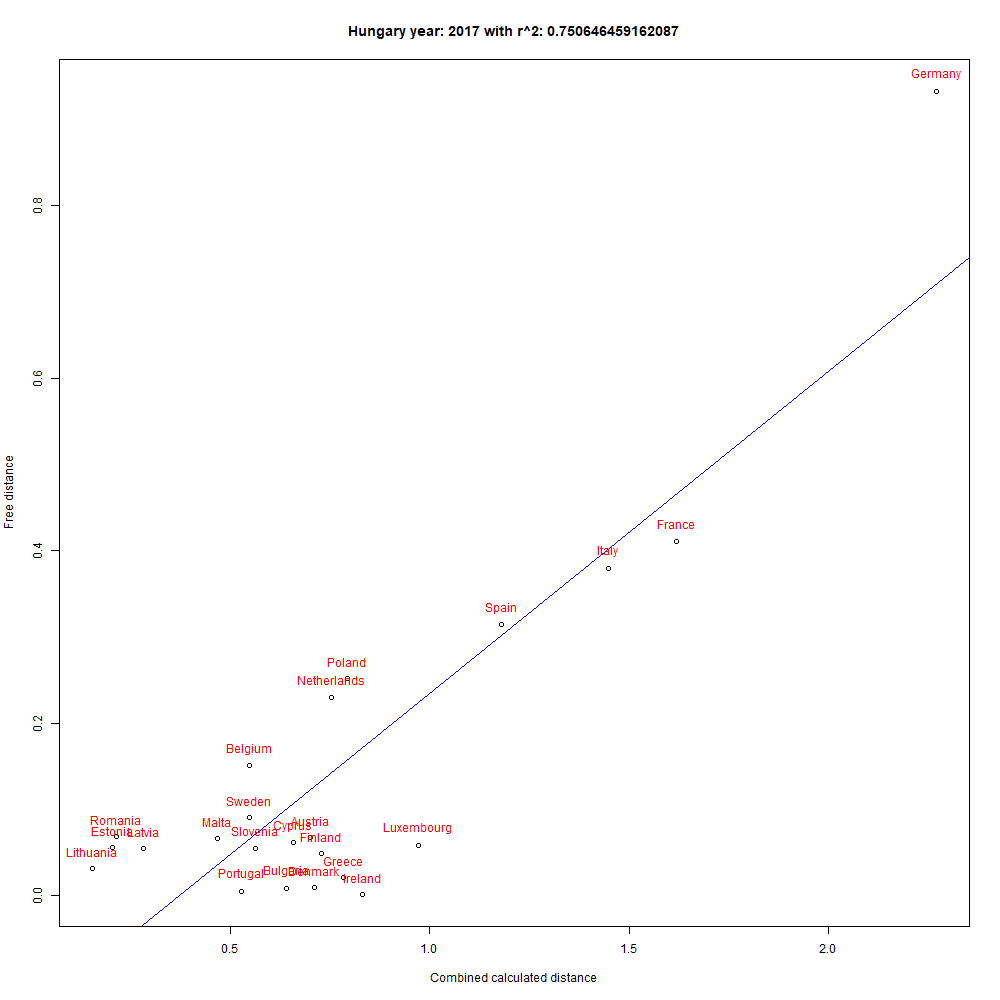
\includegraphics[width = \textwidth]{images/Hungary 2017.png}
		\caption{Hungary 2017}
		\label{fig:/Hungary_2017}
	\end{figure}
	\newpage
	Το οποίο μπορούμε να το αντιπαραθέσουμε με τις 3 άλλες χώρες που είδαμε και πριν.
	
	\begin{figure}[H]
		\centering
		\begin{subfigure}[b]{0.3\textwidth}
			\centering
			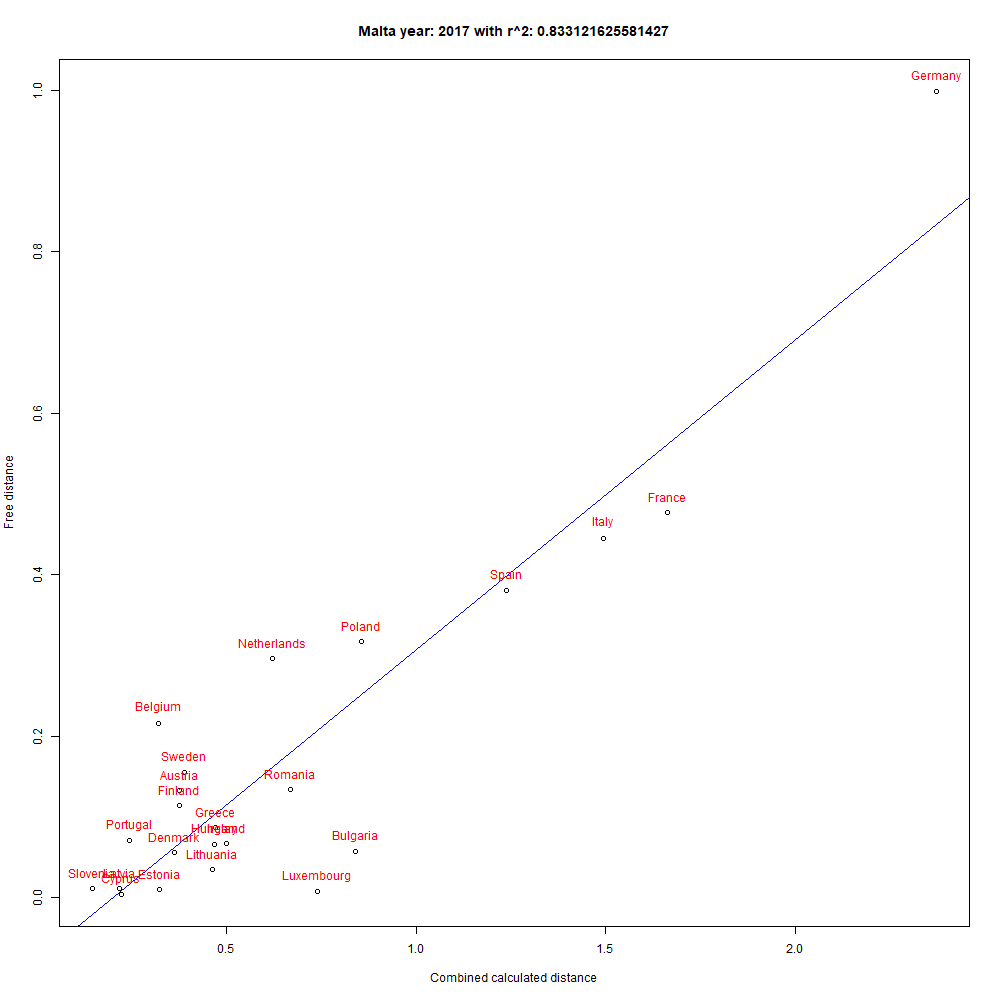
\includegraphics[width=\textwidth]{images/Malta 2017.png}
			\caption{Malta 2017}
			\label{fig:Malta_2017}
		\end{subfigure}
		\hfill
		\begin{subfigure}[b]{0.3\textwidth}
			\centering
			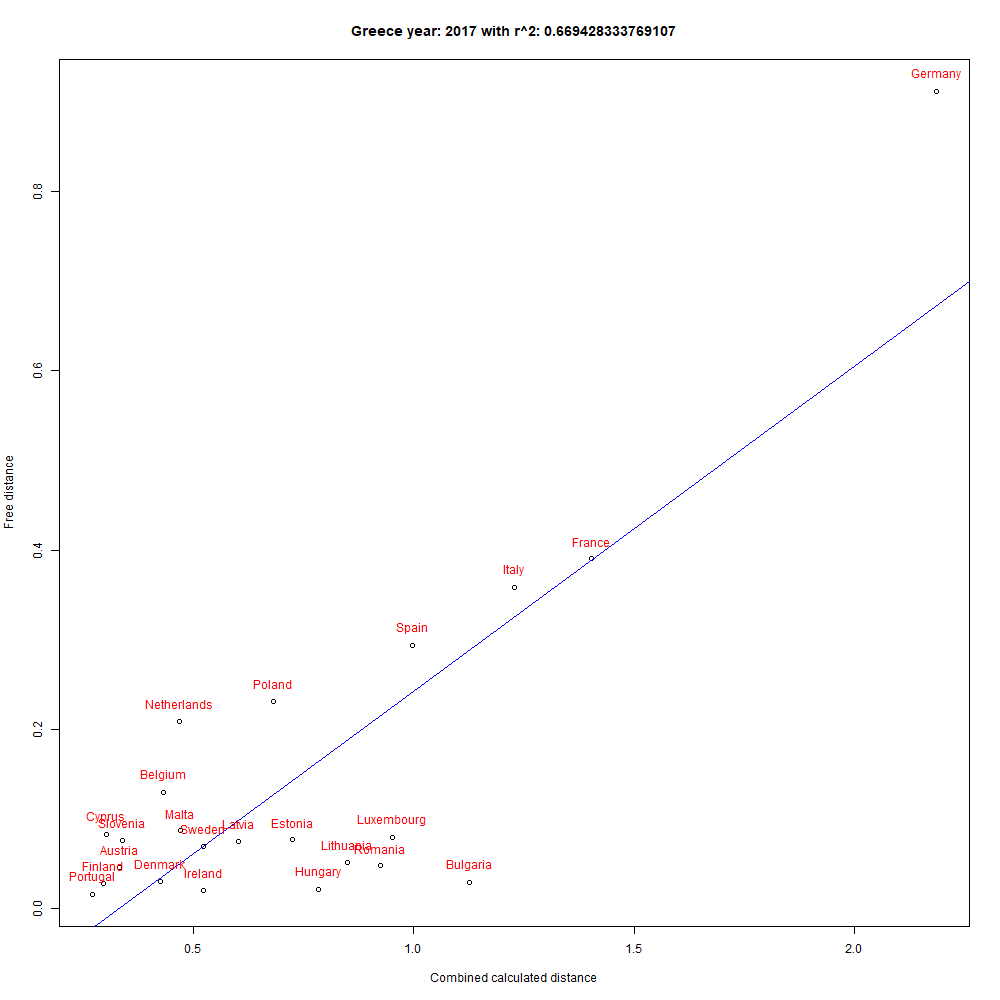
\includegraphics[width=\textwidth]{images/Greece 2017.png}
			\caption{Greece 2017}
			\label{fig:Greece_2017}
		\end{subfigure}
		\hfill
		\begin{subfigure}[b]{0.3\textwidth}
			\centering
			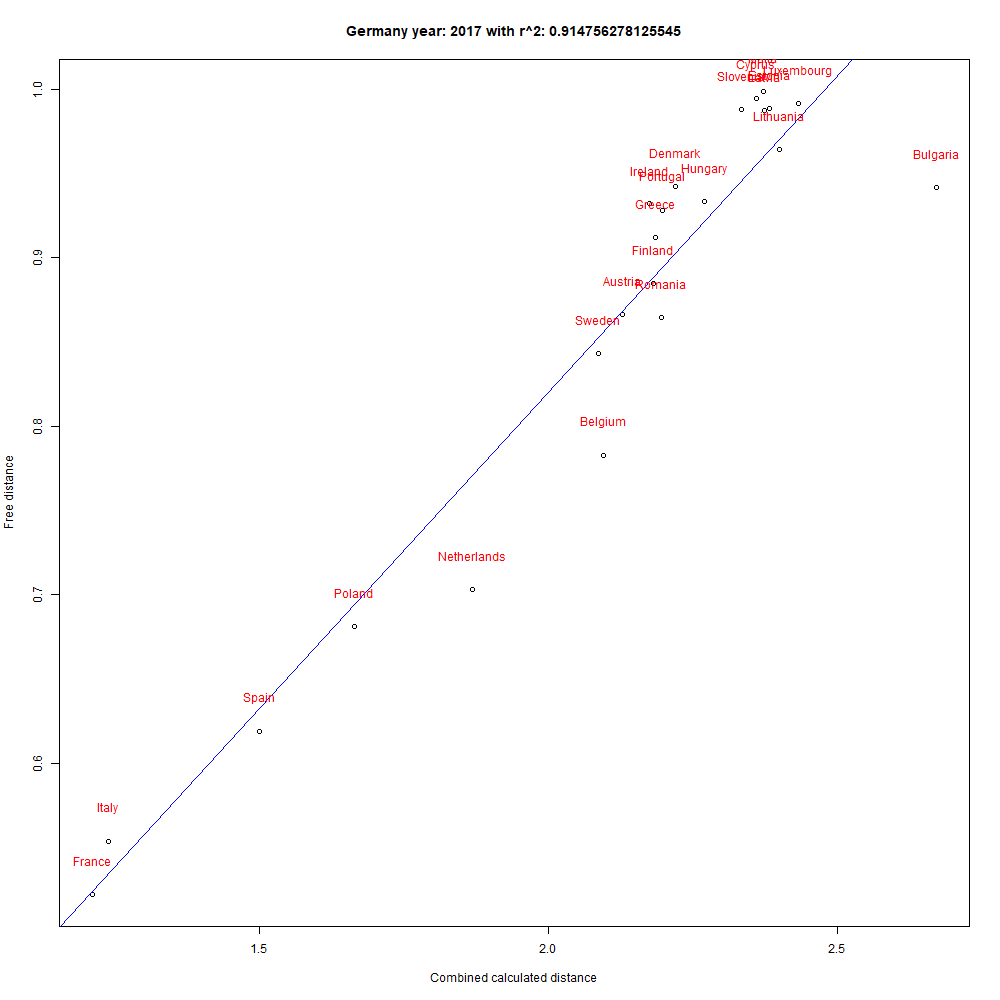
\includegraphics[width=\textwidth]{images/Germany 2017.png}
			\caption{Germany 2017}
			\label{fig:Germany_2017}
		\end{subfigure}
		%\caption{Αποστάσεις χωρών σε heatmap}
		\label{fig:3_examples}
	\end{figure}
	
	Παράλληλα μπορούμε να δούμε μέσα στις χρονιές επαναλαμβάνοντας το ίδιο πείραμα για όλες τις χώρες, τι θα προκύψει. 
	
	\begin{table}[ht]
		\centering
		\begin{tabular}{r|rrrrr}
			\hline
			year & slope & mean r\_squared & min\_r\_squared & max\_r\_squared \\
			\hline
			2008 & 0.34 & 0.65 & 0.00 & 0.79 \\
			2009 & 0.32 & 0.60 & 0.02 & 0.78 \\
			2010 & 0.33 & 0.58 & 0.04 & 0.79 \\
			2011 & 0.33 & 0.62 & 0.04 & 0.78 \\
			2012 & 0.34 & 0.64 & 0.07 & 0.82 \\
			2013 & 0.37 & 0.72 & 0.51 & 0.92 \\
			2014 & 0.36 & 0.71 & 0.46 & 0.93 \\
			2015 & 0.37 & 0.75 & 0.48 & 0.94 \\
			2016 & 0.35 & 0.70 & 0.50 & 0.91 \\
			2017 & 0.36 & 0.73 & 0.47 & 0.91 \\
			2018 & 0.37 & 0.74 & 0.43 & 0.92 \\
			\hline
		\end{tabular}
	\end{table}
	Συμπεράσματα:
	\begin{itemize}
		\item Η κλίση αυτής της ευθείας δείχνει να παραμένει πολύ σταθερή
		\item Μέχρι το 2012 (δηλαδή και το τέλος της φάσης ΙΙ) βλέπουμε πως υπάρχουν χώρες για τις οποίες δεν ισχύει το συμπέρασμα το οποίο είχαμε βγάλει, περί δικαιότητας του συστήματος.
		\item Μετά τη φάση ΙΙΙ ακόμα υπάρχουν χώρες για τις οποίες η μέθοδος αυτή δε δίνει σημαντικά καλές τιμές. 
	\end{itemize}
	\newpage
	
	Ένα ερώτημα που νομίζω πως είναι λογικό να προκύψει ξαφνικά είναι το "ποιο κρητήριο κάνει μία χώρα να είναι κατάλληλη για αυτή τη δουλειά; Πότε μπορούμε να διαλέξουμε μία χώρα για να είναι χρήσιμες οι αποστάσεις της;". Οπότε τα βάζουμε όλα μαζί στο ίδιο γράφημα και έχουμε:
	
	\begin{figure}[H]
		\centering
		
\includegraphics[width = \textwidth]{images/2017 r^2 vs GDP.png}
		\caption{2017 r\^2 vs GDP}
		\label{fig:/2017 r^2 vs GDP}
	\end{figure}
	
	Δοκιμάζοντας και άλλα χαρακτηριστικά δεν κατέληξα σε κάτι πιο ενδιαφέρον από το παραπάνω διάγραμμα. Η Γερμανία δείχνει να είναι πολύ καλή για να κάνουμε αυτή τη δουλειά, μάλλον γιατί στον "χώρο των αποστάσεων" είναι τόσο μακριά από όλους τους άλλους που οι υπόλοιποι καταλήγουν να είναι συγκριτικά κοντά. Αυτό το λέω σαν διαισθητική παρατήρηση, δεν ξέρω αν στηρίζεται μαθηματικά. 
	
	Το επόμενο βήμα είναι να δούμε το προηογούμενο με τα βέλτιστα βάρη. 
	
	\section{ΓιΑ την 28η Φεβρουαρίου}
	
	Την τελευταία φορά προτείναμε να κάνουμε/δούμε/διαβάσουμε, χωρίς κάποια σειρά:
	\begin{enumerate}
		\item Να διαβάσω τον αλγόριθμο του benchmark, πώς προκύπτει ακριβώς.
		\item Να εξετάσουμε αν τα αποτελέσματα σχετικά με το "ποιες χώρες εξηγούν καλύτερα τα δεδομένα είναι consistant μέσα στον χρόνο.
		\item Υπάρχει κάποιο clustering μεταξύ των χωρών που εξηγούν καλά ή κακά τις άλλες χώρες; Έχουν κάποια κοινά χαρακτηριστικά όλες αυτές;
		\item Γιατί είναι η Ολλανδία τόσο διαφορετική;
		\item Να επαναληφθούν οι δοκιμές της προηγούμενη φοράς, αλλά για τις φάσεις 1,2 ( πιθανώς θα προκύψει πρόβλημα με τα δεδομένα για αυτές τις περιόδους, αλλά θα το δούμε)
		\item Κάνε δοκιμές και με μία fictional χώρα η οποία να έχει ως τιμές της μόνο τα medians όλων των χωρών. 
		\item Να γίνει καλύτερα η σύγκριση μεταξύ κάθε δύο παλινδρομήσεων, αξιολογώντας και το $r^2$, αλλά και άλλες παραμέτρους, όπως το p-value και MSE/MAE.
		\item Τι συμβαίνει στα πρώτα χρόνια με την Πολωνία και την Γαλλία;
		\item Να χρησιμοποιηθεί ggplot για τα δραγράμματα και να έχουν πάντα grid.
		\item Για διάβασμα : A multi-xriteria decision analysis model for carbon emission quota allocation in China's east coastal areas: Efficiency and Equity.
		
	\end{enumerate}
	
	\subsection{Αλλαγή 1}
	Το πρώτο βήμα που έγινε είναι το να ξαναγίνουν πολλά από τα πειράματα, μόνο που αυτή τη φορά, για να θεωρηθεί μία γραμμική παλινδρόμηση καλύτερη από μία άλλη, θα πρέπει να είναι αληθή τα παρακάτω κριτήρια:
	\begin{itemize}
		\item Εχει μεγαλύτερο $r^2$.
		\item Έχει p-value μικρότερο του 0.05.
		\item To Mean Square Error δεν είναι πολύ μεγαλύτερο από την προηγούμενη μέγιστη τιμή (1.5 φορά).
	\end{itemize}
	
	\subsection{Μεσαία χώρα ανά τα έτη}
	Εδώ βλέπουμε την πιο μεσαία χώρα κάθε χρονιάς και το πόσο καλά αποδίδει στο να εξηγεί τις άλλες χώρες. Οι τιμές στο p-value βγήκαν όντως 0, η μεγαλύτερη είχε την τιμή 0.00002581...
	\begin{table}[H]
		\centering
		\begin{tabular}{r|rrrrl}
			\hline
			Year & R\verb|^|2 & p-value & MSE & Country \\
			\hline
			2008 & 0.77 & 0.00 & 0.01 & Denmark \\ 
			2009 & 0.69 & 0.00 & 0.01 & Denmark \\
			2010 & 0.57 & 0.00 & 0.01 & Greece \\
			2011 & 0.65 & 0.00 & 0.02 & Denmark \\
			2012 & 0.75 & 0.00 & 0.01 & Ireland \\
			2013 & 0.71 & 0.00 & 0.01 & Portugal \\
			2014 & 0.58 & 0.00 & 0.02 & Hungary \\ 
			2015 & 0.77 & 0.00 & 0.01 & Portugal \\
			2016 & 0.70 & 0.00 & 0.01 & Portugal \\
			2017 & 0.75 & 0.00 & 0.01 & Hungary \\
			2018 & 0.74 & 0.00 & 0.01 & Hungary \\ 
			\hline
		\end{tabular}
	\end{table}
	\subsection{Όλες οι χώρες για όλα τα έτη}
	
	
	\begin{table}[H]
		\centering
		\tabcolsep=0.11cm
		\begin{tabular}{rrrrrrrrrrrrrr}
			\hline
			& 2008 & 2009 & 2010 & 2011 & 2012 & 2013 & 2014 & 2015 & 2016 & 2017 & 2018 & max p-value & max MSE \\ 
			\hline
			Austria & 0.70 & 0.62 & 0.66 & 0.68 & 0.71 & 0.74 & 0.73 & 0.82 & 0.72 & 0.68 & 0.74 & 0.00 & 0.02 \\ 
			Belgium & 0.62 & 0.62 & 0.62 & 0.64 & 0.65 & 0.67 & 0.67 & 0.65 & 0.57 & 0.60 & 0.59 & 0.00 & 0.01 \\
			Bulgaria & 0.75 & 0.67 & 0.73 & 0.67 & 0.78 & 0.84 & 0.85 & 0.86 & 0.69 & 0.81 & 0.85 & 0.00 & 0.01 \\
			Cyprus & 0.79 & 0.71 & 0.69 & 0.71 & 0.78 & 0.67 & 0.58 & 0.73 & 0.72 & 0.75 & 0.78 & 0.00 & 0.02 \\ 
			Denmark & 0.77 & 0.69 & 0.61 & 0.65 & 0.74 & 0.71 & 0.72 & 0.73 & 0.72 & 0.68 & 0.69 & 0.00 & 0.02 \\
			Estonia & 0.79 & 0.74 & 0.67 & 0.69 & 0.66 & 0.64 & 0.68 & 0.78 & 0.68 & 0.82 & 0.81 & 0.00 & 0.02 \\ 
			Finland & 0.71 & 0.64 & 0.66 & 0.73 & 0.68 & 0.73 & 0.77 & 0.80 & 0.72 & 0.69 & 0.76 & 0.00 & 0.01 \\
			\rowcolor{lightgray} France & 0.08 & 0.08 & 0.20 & 0.19 & 0.25 & 0.78 & 0.79 & 0.78 & 0.78 & 0.73 & 0.76 & 0.19 & 0.01 \\
			Germany & 0.76 & 0.75 & 0.79 & 0.76 & 0.80 & 0.92 & 0.93 & 0.94 & 0.91 & 0.91 & 0.92 & 0.00 & 0.01 \\
			Greece & 0.62 & 0.57 & 0.57 & 0.60 & 0.57 & 0.51 & 0.46 & 0.69 & 0.65 & 0.67 & 0.71 & 0.00 & 0.02 \\ 
			Hungary & 0.74 & 0.52 & 0.58 & 0.69 & 0.69 & 0.67 & 0.58 & 0.78 & 0.73 & 0.75 & 0.74 & 0.00 & 0.02 \\
			Ireland & 0.70 & 0.76 & 0.47 & 0.70 & 0.75 & 0.73 & 0.69 & 0.77 & 0.73 & 0.63 & 0.64 & 0.00 & 0.02 \\
			Italy & 0.63 & 0.61 & 0.65 & 0.64 & 0.60 & 0.86 & 0.82 & 0.75 & 0.74 & 0.72 & 0.78 & 0.00 & 0.01 \\ 
			Latvia & 0.76 & 0.70 & 0.62 & 0.66 & 0.68 & 0.77 & 0.74 & 0.75 & 0.78 & 0.84 & 0.81 & 0.00 & 0.02 \\
			Lithuania & 0.77 & 0.78 & 0.63 & 0.70 & 0.74 & 0.79 & 0.76 & 0.74 & 0.74 & 0.79 & 0.81 & 0.00 & 0.02 \\
			Luxembourg & 0.79 & 0.67 & 0.59 & 0.77 & 0.73 & 0.68 & 0.65 & 0.75 & 0.60 & 0.74 & 0.70 & 0.00 & 0.02 \\ 
			Malta & 0.76 & 0.65 & 0.62 & 0.68 & 0.78 & 0.75 & 0.72 & 0.82 & 0.71 & 0.83 & 0.82 & 0.00 & 0.02 \\
			Netherlands & 0.51 & 0.53 & 0.53 & 0.44 & 0.54 & 0.60 & 0.60 & 0.51 & 0.50 & 0.47 & 0.43 & 0.00 & 0.01 \\
			\rowcolor{lightgray} Poland & 0.00 & 0.02 & 0.04 & 0.04 & 0.07 & 0.60 & 0.60 & 0.48 & 0.54 & 0.69 & 0.69 & 0.92 & 0.02 \\
			Portugal & 0.71 & 0.66 & 0.66 & 0.60 & 0.59 & 0.71 & 0.73 & 0.77 & 0.70 & 0.75 & 0.77 & 0.00 & 0.02 \\ 
			Romania & 0.53 & 0.46 & 0.42 & 0.58 & 0.45 & 0.60 & 0.75 & 0.80 & 0.64 & 0.66 & 0.67 & 0.00 & 0.01 \\
			Slovenia & 0.78 & 0.59 & 0.59 & 0.67 & 0.70 & 0.76 & 0.73 & 0.77 & 0.78 & 0.78 & 0.81 & 0.00 & 0.02 \\ 
			Spain & 0.63 & 0.61 & 0.63 & 0.57 & 0.60 & 0.84 & 0.74 & 0.76 & 0.72 & 0.77 & 0.81 & 0.00 & 0.01 \\
			Sweden & 0.70 & 0.56 & 0.61 & 0.59 & 0.67 & 0.74 & 0.75 & 0.81 & 0.75 & 0.77 & 0.77 & 0.00 & 0.02 \\ 
			United Kingdom & 0.75 & 0.71 & 0.77 & 0.78 & 0.82 & 0.63 & 0.69 & 0.66 & 0.66 & 0.72 & 0.71 & 0.00 & 0.01 \\
			\hline
		\end{tabular}
	\end{table}
	Το οποίο γραφικά φαίνεται και ως εξής:
	\begin{figure}[H]
		\centering
		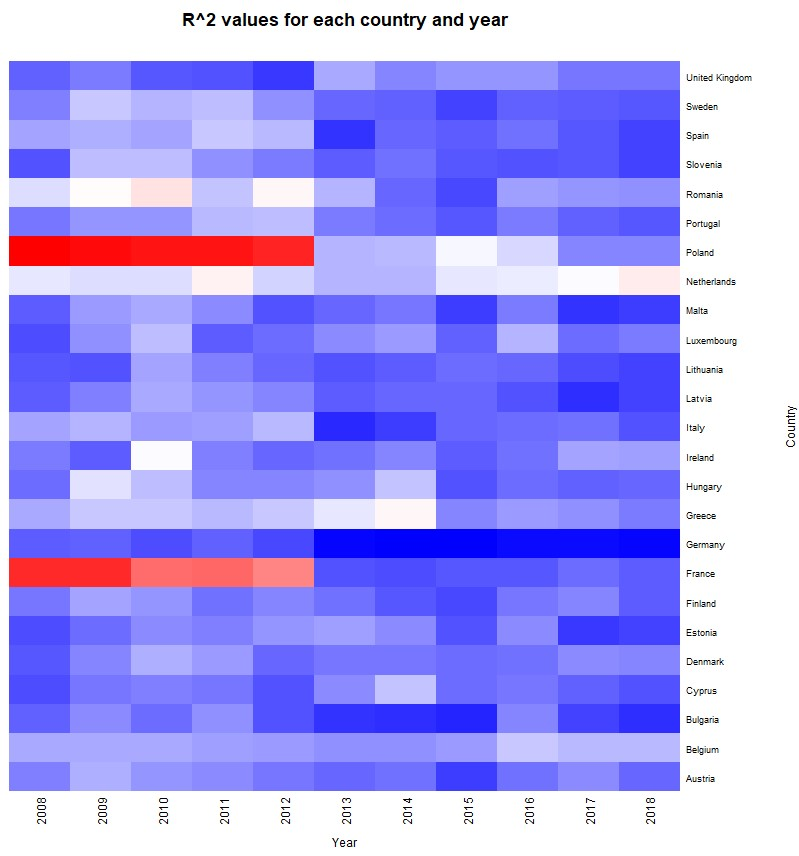
\includegraphics[width = \textwidth]{images/plot.jpg}
		\caption{$r^2$}
		\label{fig:/2017 r^2 vs GDP}
	\end{figure}
	
	Το πιο λογικό λοιπόν βήμα είναι το να ελέγξουμε το γιατί αυτές οι δύο χώρες αλλάζουν τόσο πολύ το 2013. Οπότε ας δούμε τα δεδομένα που χρησιμοποιούμε για αυτές:
	\begin{table}[H]
		\centering
		\begin{tabular}{rllll}
			\hline
			& 2012 & 2013 & 2012 & 2013 \\
			\hline
			GEO & Poland & Poland & France & France \\
			Total\_energy\_supply & 0.3083121 & 0.3038433 & 0.8215192 & 0.8080548 \\ 
			GDPpc & 0.1163326 & 0.1141371 & 0.3630366 & 0.3550416 \\
			Population & 0.4732704 & 0.4716958 & 0.8164021 & 0.8183792 \\
			Inflation & 0.57990986 & 0.07563843 & 0.28530815 & 0.19301719 \\ 
			Verified\_emissions & 0.4212666 & 0.4212431 & 0.2421093 & 0.2422275 \\
			Agriculture & 0.3402106 & 0.3644831 & 1.0000000 & 0.8928814 \\
			Industry & 0.1558893 & 0.1482026 & 0.4982965 & 0.5053396 \\
			Manufacturing & 0.1166064 & 0.1091561 & 0.3911272 & 0.3913494 \\ 
			\hline
		\end{tabular}
	\end{table}
	Όπως είναι εμφανές, στα δεδομένα των χωρών δεν υπάρχει κάτι προφανές το οποίο να δικαιολογεί αυτήν την τόσο απότομη αλλαγή. Τα δεδομένα τα βλέπουμε κανονικοποιημένα.
	
	Επίσης, για το ποιες χώρες τα πηγαίνουν καλύτερα, μπορούμε ν αφτιάξουμε αυτήν την κατάταξη, η οποία είναι αρκετά αντιπροσωπευτική.
	\begin{table}[H]
		\centering
		\begin{tabular}{rlr}
			\hline
			& Country & Average R\verb|^|2 \\
			\hline
			1 & Germany & 0.85 \\
			2 & Bulgaria & 0.77 \\
			3 & Lithuania & 0.75 \\
			4 & Malta & 0.74 \\
			5 & Latvia & 0.74 \\ 
			6 & Estonia & 0.72 \\
			7 & Slovenia & 0.72 \\
			8 & Cyprus & 0.72 \\
			9 & United Kingdom & 0.72 \\
			10 & Finland & 0.72 \\
			11 & Italy & 0.71 \\
			12 & Austria & 0.71 \\
			13 & Sweden & 0.70 \\ 
			14 & Denmark & 0.70 \\
			15 & Spain & 0.70 \\
			16 & Luxembourg & 0.70 \\
			17 & Portugal & 0.70 \\
			18 & Ireland & 0.69 \\
			19 & Hungary & 0.68 \\
			20 & Belgium & 0.63 \\
			21 & Greece & 0.60 \\
			22 & Romania & 0.60 \\
			23 & Netherlands & 0.52 \\
			24 & France & 0.49 \\ 
			25 & Poland & 0.34 \\
			\hline
		\end{tabular}
	\end{table}

	\newpage
	\section{Για τη 14η Φλεβάρη}
	
	Είπαμε να διορθωθούν τα παρακάτω:
	\begin{itemize}
		\item Οι πίνακες με δεδομένα να έχουν 2 δεκαδικά ψηφία ή όσα είναι αναγκαία, όχι παραπάνω.
		\item Να προστίθενται γραμμές στις αναφορές ανά 5 στοιχεία, ώστε να είναι ευδιάκριτα τα νούμερα.
		\item Να φτιαχτεί ένα πινακάκι με descriptive statistics για τα δεδομένα τα οποία έχουμε, να περιλαμβάνει min, max, quantiles, median και boxplot.
		\item Να γίνει η παραπάνω παρουσίαση για τα αρχικά δεδομένα, αλλά και για τα κανονικοποιημένα δεδομένα.
		\item Πιθανώς να δούμε την διαφορά που θα είχε η χρήση κάποιου διαφορετικού τρόπου κανονικοποίησης. (Μέχρι τώρα η κανονικοποίηση γίνεται διαιρώντας με την μέγιστη τιμή. Ένας άλλος τρόπος θα ήταν ο $\frac{X- X_{min}}{X_{max}- X_{min}}$)
	\end{itemize}
	
	
	\subsection{Πίνακας $r^2$ με βέλτιστα επιλεγμένα βάρη}
	Εδώ φαίνεται ο πίνακας της προηγούμενης εβδομάδας, με την διαφορά ότι κάθε χώρα μπορούσε να επιλέξει το "mix" δεδομένων που θα χρησιμοποιήσει ώστε να είναι βέλτιστο το $r^2$. Εδώ βλέπουμε πως η Γαλλία έχει  πολύ πιο μικρό πρόβλημα. 
	
	Ο αλγόριθμος ο οποίος χρησιμοποιήθηκε για να βγει αυτός ο πίνακας είναι πολύ κακός. Θεωρεί πως υπάρχει κάποια γραμμική συσχέτιση της ικανότητας μίας χώρας να περιγράψει τις άλλες και του βάρους κάθε διαφορετικού δεδομένου (για παράδειγμα, τα verfied emissions έχουν μία γνησίως αύξουσα σχέση με την ικανότητα της χώρας να περιγράψει τις άλλες.) Αυτό δεν ισχύει και ίσως είναι ενδιαφέρον το να δούμε πώς μοιάζει η συνάρτηση αυτή. 
	
	Πάντως ο αλγόριθμος αυτός κάνει τα παρακάτω:
	\begin{enumerate}
		\item Διαλέγει ένα από τα βάρη των διαφορετικών δεδομένων.
		\item Δοκιμαστικά "ανεβάζει" και "κατεβάζει" το αντίστοιχο βάρος και βλέπει ποιο οδηγεί σε καλύτερη παλινδρόμηση.
		\item Επαναλαμβάνει το προηγούμενο βήμα μέχρι να χτηπίσει κάποιο όριο ή να είναι χειρότερες και οι δύο επιλογές.
		\item Προχωρά στο επόμενο βάρος το οποίο μπορεί να βελτιστοποιήσει.
		\item Οι παράμετροι ήταν:
		\begin{itemize}
			\item Ελάχιστο βάρος: 0
			\item Μέγιστο βάρος: 1000
			\item Βήμα: 10
			\item Τιμή εκκίνησης: 50
			\item Υπάρχουν 8 βάρη, τυχαία διαλέγει το βάρος το οποίο θα προσπαθήσει να βελτιστοποιήσει 100 φορές 
		\end{itemize}
	\end{enumerate}
	 
	\begin{table}[H]
		\centering
		\tabcolsep=0.11cm
		\begin{tabular}{r|rrrrr|rrrrrr|rr}
			\hline
			& 2008 & 2009 & 2010 & 2011 & 2012 & 2013 & 2014 & 2015 & 2016 & 2017 & 2018 & max p-value & max MSE \\ 
			\hline
			Austria & 0.99 & 0.98 & 0.98 & 0.98 & 0.99 & 0.98 & 0.98 & 0.98 & 0.98 & 0.97 & 0.97 & 0.00 & 0.00 \\ 
			Belgium & 0.98 & 0.98 & 0.98 & 0.99 & 0.98 & 0.91 & 0.90 & 0.91 & 0.89 & 0.88 & 0.89 & 0.00 & 0.00 \\ 
			Bulgaria & 0.98 & 0.98 & 0.98 & 0.98 & 0.99 & 0.97 & 0.97 & 0.97 & 0.97 & 0.97 & 0.97 & 0.00 & 0.00 \\ 
			Cyprus & 0.99 & 0.98 & 0.98 & 0.98 & 0.99 & 0.97 & 0.96 & 0.97 & 0.97 & 0.97 & 0.97 & 0.00 & 0.00 \\ 
			Denmark & 0.99 & 0.98 & 0.97 & 0.98 & 0.99 & 0.97 & 0.97 & 0.97 & 0.97 & 0.97 & 0.96 & 0.00 & 0.00 \\ 
			Estonia & 0.99 & 0.98 & 0.98 & 0.98 & 0.98 & 0.96 & 0.97 & 0.97 & 0.97 & 0.97 & 0.97 & 0.00 & 0.00 \\ 
			Finland & 0.99 & 0.98 & 0.98 & 0.98 & 0.98 & 0.97 & 0.98 & 0.97 & 0.98 & 0.97 & 0.97 & 0.00 & 0.00 \\ 
			\rowcolor{cyan} France & 0.08 & 0.08 & 0.97 & 0.96 & 0.98 & 0.98 & 0.98 & 0.96 & 0.98 & 0.98 & 0.98 & 0.19 & 0.01 \\ 
			Germany & 1.00 & 0.99 & 0.99 & 0.99 & 0.99 & 0.98 & 0.98 & 0.98 & 0.98 & 0.97 & 0.98 & 0.00 & 0.00 \\ 
			Greece & 0.98 & 0.98 & 0.98 & 0.98 & 0.98 & 0.96 & 0.96 & 0.97 & 0.98 & 0.97 & 0.97 & 0.00 & 0.00 \\ 
			Hungary & 0.99 & 0.97 & 0.97 & 0.98 & 0.98 & 0.97 & 0.96 & 0.97 & 0.97 & 0.97 & 0.97 & 0.00 & 0.00 \\ 
			Ireland & 0.99 & 0.98 & 0.97 & 0.99 & 0.99 & 0.97 & 0.97 & 0.97 & 0.97 & 0.96 & 0.96 & 0.00 & 0.00 \\ 
			Italy & 0.96 & 0.93 & 0.97 & 0.98 & 0.99 & 0.96 & 0.96 & 0.97 & 0.97 & 0.97 & 0.96 & 0.00 & 0.00 \\ 
			Latvia & 0.98 & 0.98 & 0.97 & 0.98 & 0.98 & 0.97 & 0.97 & 0.97 & 0.98 & 0.98 & 0.97 & 0.00 & 0.00 \\ 
			Lithuania & 0.99 & 0.98 & 0.97 & 0.98 & 0.99 & 0.98 & 0.98 & 0.98 & 0.98 & 0.98 & 0.97 & 0.00 & 0.00 \\ 
			Luxembourg & 0.98 & 0.97 & 0.97 & 0.98 & 0.98 & 0.96 & 0.96 & 0.97 & 0.97 & 0.97 & 0.97 & 0.00 & 0.00 \\ 
			Malta & 0.99 & 0.98 & 0.97 & 0.98 & 0.99 & 0.97 & 0.97 & 0.97 & 0.97 & 0.98 & 0.97 & 0.00 & 0.00 \\ 
			Netherlands & 0.97 & 0.97 & 0.97 & 0.97 & 0.98 & 0.81 & 0.81 & 0.80 & 0.79 & 0.73 & 0.69 & 0.00 & 0.00 \\ 
			\rowcolor{cyan} Poland & 0.00 & 0.02 & 0.04 & 0.04 & 0.07 & 0.94 & 0.94 & 0.94 & 0.95 & 0.95 & 0.94 & 0.92 & 0.02 \\ 
			Portugal & 0.99 & 0.98 & 0.98 & 0.98 & 0.98 & 0.97 & 0.98 & 0.97 & 0.98 & 0.97 & 0.97 & 0.00 & 0.00 \\ 
			Romania & 0.95 & 0.95 & 0.93 & 0.96 & 0.96 & 0.98 & 0.98 & 0.98 & 0.97 & 0.97 & 0.97 & 0.00 & 0.00 \\ 
			Slovenia & 0.99 & 0.97 & 0.97 & 0.98 & 0.98 & 0.97 & 0.97 & 0.97 & 0.97 & 0.97 & 0.97 & 0.00 & 0.00 \\ 
			Spain & 0.98 & 0.97 & 0.98 & 0.97 & 0.98 & 0.95 & 0.94 & 0.95 & 0.95 & 0.95 & 0.95 & 0.00 & 0.00 \\ 
			Sweden & 0.99 & 0.98 & 0.97 & 0.98 & 0.99 & 0.97 & 0.98 & 0.98 & 0.97 & 0.97 & 0.97 & 0.00 & 0.00 \\ 
			United Kingdom & 0.99 & 0.99 & 0.99 & 0.99 & 0.99 & 0.92 & 0.94 & 0.97 & 0.98 & 0.98 & 0.98 & 0.00 & 0.00 \\ 
			\hline
		\end{tabular}
	\end{table}
	Σε αυτόν τον πίνακα τα μέσα βάρη ήταν:
	\begin{itemize}
		\item Population: 59.63
		\item GDP per capita: 19.85
		\item Inflation: 15.12
		\item Agriculture: 69.09
		\item Industry: 407.60
		\item Manufacturing: 12.69
		\item Total energy supply: 170.25
		\item Verified emissions: 849.81\\
	\end{itemize}
\newpage
\subsection{Οπτικοποίηση δεδομένων}
\subsubsection{Πληθυσμός}
Για τον πληθυσμό δεν έχω τίποτα εντυπωσιακό να πω. Ίσως είναι κάπως εύκολο να δούμε όλα τα δεδομένα ταυτόχρονα και να παρατηρήσουμε τι αλλαγή επιφέρει η κανονικοποίηση στα δεδομένα. Όπως φαίνεται στα figure 7 και 8. Τα σχήματα είναι ολόιδια. Η διαφορά είναι πως το ένα έχει διαιρεθεί με το 1000000 ενώ το άλλο έχει διαιρεθεί με το μέγιστο κάθε χρονιάς, οπότε είναι ελαφρώς διαφορετικές οι σχέσεις μεταξύ των αριθμών κάθε χώρας. 

Παράλληλα, μπορούμε να παρατηρήσουμε τα δεδομένα κάπως καλύτερα:



\begin{figure}[H]
	\centering
	\includegraphics[width=1\linewidth]{"images/Boxplot Population Normalized vs Country"}
	\caption{}
	\label{fig:boxplot-population-normalized-vs-country}
\end{figure}
\begin{figure}[H]
	\centering
	\includegraphics[width=1\linewidth]{"images/Boxplot Population in Millions vs Country"}
	\caption{}
	\label{fig:boxplot-population-in-millions-vs-country}
\end{figure}

	
	
	
\end{document}	